%%
%% Copyright 2007, 2008, 2009 Elsevier Ltd
%%
%% This file is part of the 'Elsarticle Bundle'.
%% ---------------------------------------------
%%
%% It may be distributed under the conditions of the LaTeX Project Public
%% License, either version 1.2 of this license or (at your option) any
%% later version.  The latest version of this license is in
%%    http://www.latex-project.org/lppl.txt
%% and version 1.2 or later is part of all distributions of LaTeX
%% version 1999/12/01 or later.
%%
%% The list of all files belonging to the 'Elsarticle Bundle' is
%% given in the file `manifest.txt'.
%%

%% Template article for Elsevier's document class `elsarticle'
%% with numbered style bibliographic references
%% SP 2008/03/01

\documentclass[preprint,12pt]{elsarticle}
%\documentclass[final,5p,times,twocolumn]{elsarticle}

%% Use the option review to obtain double line spacing
%% \documentclass\cite{authoryear,preprint,review,12pt]{elsarticle}

%% Use the options 1p,twocolumn; 3p; 3p,twocolumn; 5p; or 5p,twocolumn
%% for a journal layout:
%% \documentclass\cite{final,1p,times]{elsarticle}
%% \documentclass\cite{final,1p,times,twocolumn]{elsarticle}
%% \documentclass\cite{final,3p,times]{elsarticle}
%% \documentclass\cite{final,3p,times,twocolumn]{elsarticle}
%% \documentclass\cite{final,5p,times]{elsarticle}
%% \documentclass\cite{final,5p,times,twocolumn]{elsarticle}

%% For including figures, graphicx.sty has been loaded in
%% elsarticle.cls. If you prefer to use the old commands
%% please give \usepackage{epsfig}

%% The amssymb package provides various useful mathematical symbols
\usepackage{amssymb}
%% The amsthm package provides extended theorem environments
%% \usepackage{amsthm}

%% The lineno packages adds line numbers. Start line numbering with
%% \begin{linenumbers}, end it with \end{linenumbers}. Or switch it on
%% for the whole article with \linenumbers.
 \usepackage{lineno}
 \usepackage{color, soul}

\journal{International Journal of Human-Computer Studies}

\begin{document}
\linenumbers
\begin{frontmatter}

%% Title, authors and addresses

%% use the tnoteref command within \title for footnotes;
%% use the tnotetext command for theassociated footnote;
%% use the fnref command within \author or \address for footnotes;
%% use the fntext command for theassociated footnote;
%% use the corref command within \author for corresponding author footnotes;
%% use the cortext command for theassociated footnote;
%% use the ead command for the email address,
%% and the form \ead\cite{url} for the home page:
%% \title{Title\tnoteref{label1}}
%% \tnotetext[label1]{}
%% \author{Name\corref{cor1}\fnref{label2}}
%% \ead{email address}
%% \ead[url]{home page}
%% \fntext[label2]{}
%% \cortext[cor1]{}
%% \address{Address\fnref{label3}}
%% \fntext[label3]{}

\title{A Sense of Ice and Fire: Exploring Thermal Feedback with Multiple Thermoelectric-cooling Elements on a Smart Ring}

%% use optional labels to link authors explicitly to addresses:

%\address[scm1]{School of Creative Media, City University of Hong Kong}
\author[scm1]{Kening Zhu\corref{cor1}}
\author[scm1]{Taizhou Chen}
\author[scm1]{Shaoyu Cai}
\author[nus2]{Simon Perrault}
\author[kmd]{Roshan Lalintha Peiris}
%\address[label1]{School of Creative Media, City University of Hong Kong}

\address[scm1]{School of Creative Media, City University of Hong Kong, Hong Kong}
\address[nus2]{Yale-NUS College, Singapore}
\address[kmd]{Keio University Graduate School of Media Design, Keio University, Japan}
\cortext[cor1]{Corresponding author}
%\author{Kening Zhu, Taizhou Chen, Shaoyu Cai, Simon Perrault, Roshan Lalintha Peiris}

%\address{}

\begin{abstract}
%% Text of abstract
%In this paper, we investigate the use of thermal feedback on a smart ring with multiple thermoelectric coolers (TECs). Our prototype offers an increased expressivity with spatial thermal patterns. In a pilot study, we compared three different ring settings:  4, 6, and 8 TECs. Results showed that users could reliably recognize 4 points with cold stimulation (97.2\% accuracy) and still achieve decent accuracy with hot stimulation (82.4\% accuracy). In our main experiments, we demonstrated the use of 4 in-ring TECs to achieve two categories of spatial thermal patterns by combining two neighboring or opposite elements. The results revealed 12 thermal patterns that were reliably recognized by the participants with the accuracy averaging 87.5\%, indicating their potential usage as the in-ring thermal icons. The participants also elicited different applications, including direction cueing through neighboring patterns and artifact comparison through opposite patterns. This demonstrated interest in spatial thermal patterns in smart rings not only for notifications but also for various everyday activities.
In this paper, we investigate the use of thermal feedback on a smart ring with multiple thermoelectric coolers (TECs). Our prototype aims to offer an increased expressivity with spatial thermal patterns. In a pilot study with nine participants, we investigated the affordance of applying multiple miniature TECs in a ring-type finger device, by comparing the user perception in three different ring settings:  4, 6, and 8 TECs. Results showed that users could reliably recognize 4 single points with cold stimulation (97.2\% accuracy). In the following two main experiments, involving 24 participants in total (i.e. 12 for each experiment), we investigated the use of 4 in-ring TECs to achieve two categories of spatial thermal patterns by combining two neighboring or opposite elements. The results revealed 3 neighboring patterns and 5 opposite patterns that were reliably recognized by the participants with the accuracy above 80\%. While the follow-up experiment suggested that it could be confusing for users by combining four single-spot cold stimulations, three neighboring patterns, and five opposite patterns in the same group (average accuracy: 50.2\%), we conducted two more follow-up studies, each of which involved 12 participants, showing that the participants could identify the thermal patterns in the combined group of the single-spot cold stimulations and the neighboring patterns (average accuracy: 85.3\%), and the combined group of the single-spot cold stimulations and the opposite patterns (average accuracy: XXX\%). These results suggested the feasbility of using these two group of thermal patterns as thermal icons for information representation. We further conducted three design workshops, invovling six product/interface designers, to investigate the pontential of using these thermal patterns for different applications. The designers suggested different mappings between the given thermal patterns and the information, including direction cueing through single-spot and neighboring patterns, artifact comparison through opposite patterns, notifying incoming calls/messages from different persons with different locations and temperatures of the TECs, etc. This demonstrated interest in spatial thermal patterns in smart rings not only for notifications but also for various everyday activities.

%The results revealed 12 thermal patterns that were reliably recognized by the participants with the accuracy averaging 87.5\%, indicating their potential usage as the in-ring thermal icons.

%The participants also suggested different applications for smart rings with multiple thermal modules, including direction cueing through neighboring patterns and artifact comparison through opposite patterns. This demonstrated interest in spatial thermal patterns in smart rings not only for notifications but also for various everyday activities.
\end{abstract}

\begin{keyword}
smart ring \sep thermal feedback \sep spatial thermal sensitivity
%% keywords here, in the form: keyword \sep keyword

%% PACS codes here, in the form: \PACS code \sep code

%% MSC codes here, in the form: \MSC code \sep code
%% or \MSC\cite{2008} code \sep code (2000 is the default)

\end{keyword}

\end{frontmatter}

%% \linenumbers

%% main text
\section{Introduction}
Smart rings can be used to convey information easily and discretely. As fingers are one of the more sensitive body locations to haptic stimuli \cite{16}, smart rings are especially desirable. Potential information that can be relayed ranges from simple notifications to more complex continuous information, such as training progress \cite{3}, or even direction information. However, smart rings are limited by their size, which makes it hard to embed multiple actuators of the same type in them, such as vibration motors. Thus, previous research done in this area \cite{12,22} has primarily focused on using a single actuator. However, such systems can only convey simple information by using single-dimensional patterns, such as temporal \cite{25}, which usually affects the expressivity of the system.

Using multiple actuators allows for encoding of more complex information with spatial patterns. For example, a wristband with four or more output actuators (e.g. DC motors and vibration motors) could be used for navigation \cite{34}, or to perform more complex tasks, such as color comparison \cite{2}. However, vibrotactile feedback with multiple actuators does not seem to be a usable strategy to create spatial patterns with the form factor of smart ring, as the vibration at one location could easily vibrate the whole ring, making it hard to locate the source of vibration.

Although early studies \cite{26,27,31} on thermal localization showed that radiation-based non-contact heat was error-prone in localization due to the phenomenon of spatial thermal summation, later research suggested on-skin thermal stimuli through small thermal-haptic devices could improve the spatial acuity for tactile stimulation \cite{28}. In addition, the cold stimulations were generally more perceivable than the hot ones \cite{42}. Psychological research has also shown the phenomenon of illusional and referral thermal sensation \cite{6}, which implies that the perception of a thermal receptor could be triggered/altered by the concurrent stimulation on the other peripheral/closed-by receptors. In the field of human-computer interaction (HCI), this channel has been previously used in a wide variety of contexts, such as social activities \cite{40}, emotions \cite{35,37,41} and navigation \cite{34}. Thermal feedback is usually considered more stable to perceive in a moving or noisy situation and  more private than other modalities \cite{10}. Additionally, Roumen et al. \cite{24} showed that heat sensitivity is positively impacted by physical activity, with heat being easier to perceive during walking or running activities. In addition, the results of NotiRing indicated the need for investigating thermal's potential as an in-ring notification channel with improved thermal devices that have more immediate feedback.

While early psychological studies revealed the poor spatial acuity for thermal sensation on finger-tips \cite{43}, it is unknown how the results may alter with miniature on-skin TEC modules and the wearable form factor of ring. Previous research on thermal feedback for HCI has mainly focused on body locations such as the thenar eminence, face, and wrist \cite{7,9,10,19,20,23,39}. \colorbox{yellow}{Existing research showed the form factor of ring afforded eight positions of pin-point poking stimulation [XX]}. However, in the limited research on ring-based thermal feedback \cite{24},  multiple thermal actuators on the ring were not used. In this paper, we present a prototype of a smart ring with multiple miniature TEC elements and investigate the use of spatial thermal patterns. In the pilot study, we determined the maximum number of TECs that can be accurately recognized by participants. A configuration with four elements (see Fig.~\ref{fig:1}) yields an accuracy of XXX\% for cold stimuli and XXX\% for hot stimuli. We then designed a set of in-ring thermal patterns (Fig. \ref{fig:9} \& \ref{fig:12}) by combining two neighboring or opposite TECs, each of which can be triggered as cold, neutral, or hot. In a series of main experiments, we assessed the feasibility of accurately perceiving the combinational thermal patterns. Results revealed \colorbox{yellow}{XXX}, indicating their potential usage as in-ring thermal icons. Based on the participants' elicitations, we propose a list of applications that can elaborate these thermal patterns, such as \colorbox{yellow}{XXX}.

%10 thermal patterns that were reliably distinguished by the participants, with an accuracy averaging 86.2\%

\begin{figure}[tp]
  \centering
  %\subfigure\cite{]{\label{fig:fold1}\includegraphics[width=0.45\textwidth]{images/study_setup.png}}
  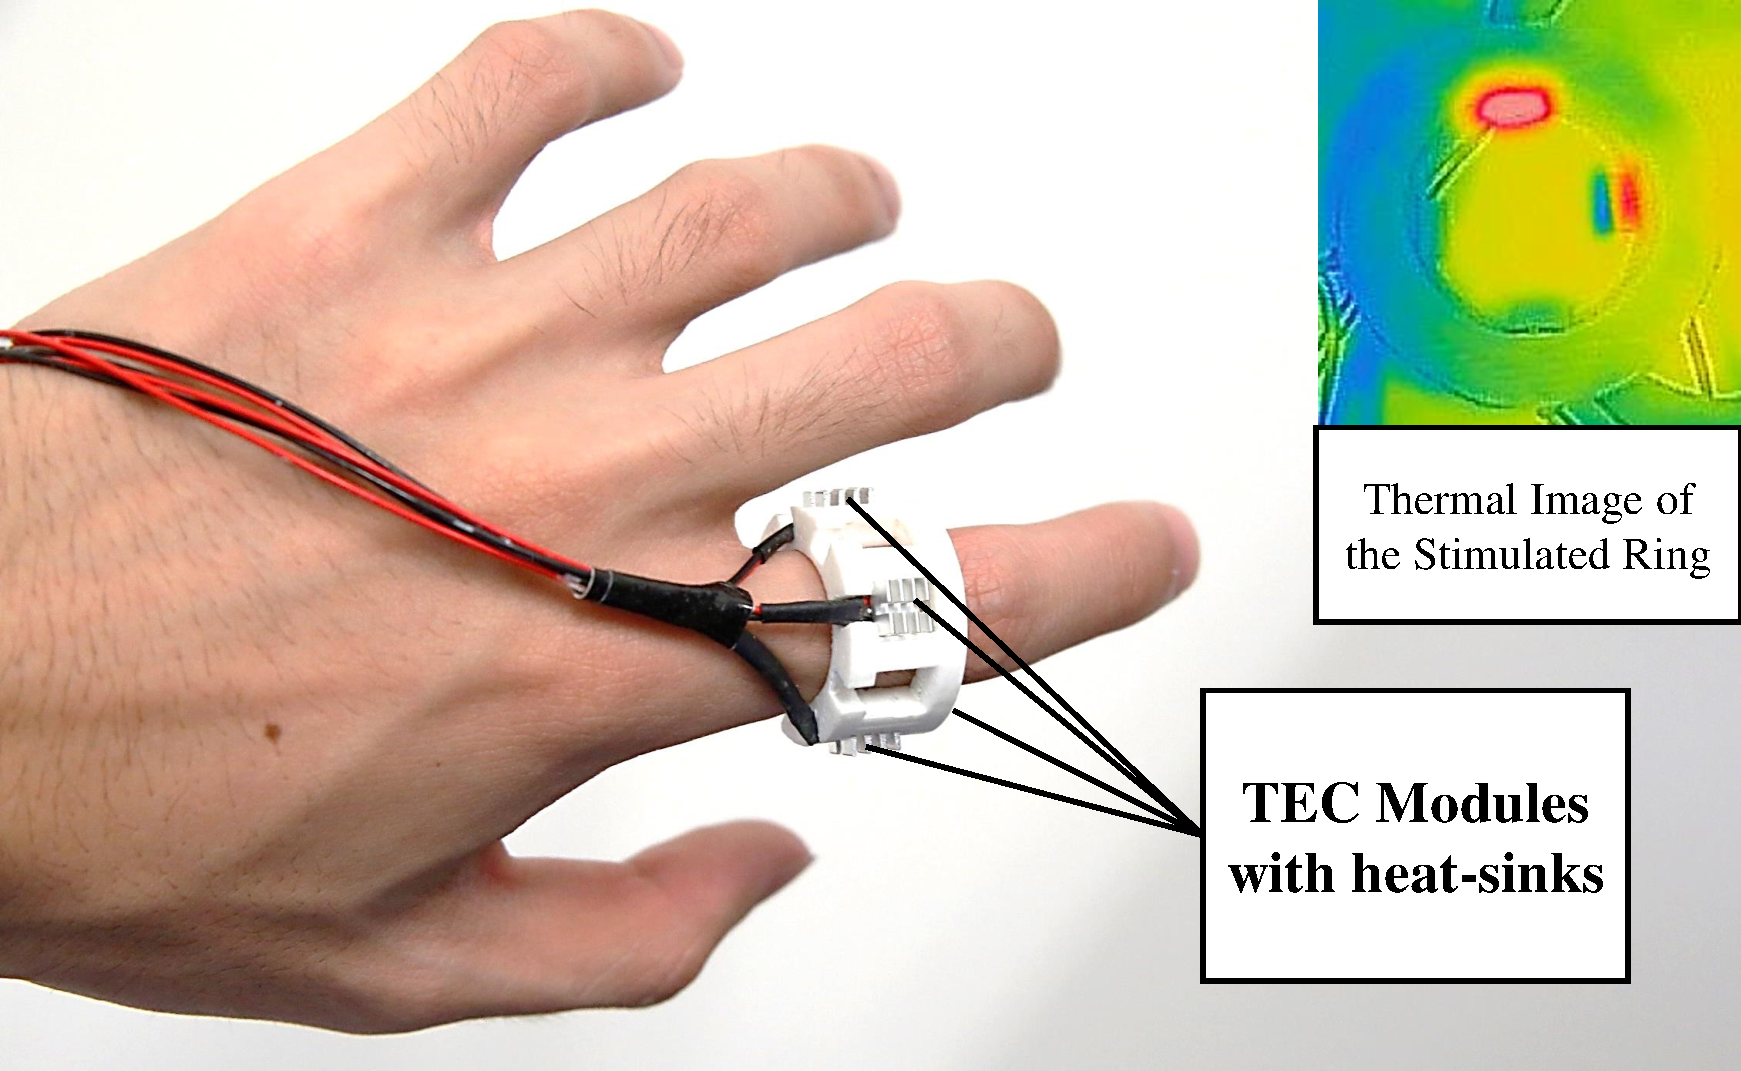
\includegraphics[width=0.8\columnwidth]{img/fig1.pdf}
  %\subfigure\cite{]{\label{fig:fold2}\includegraphics[width=0.45\textwidth]{images/wo_assembly.png}}
  \caption{Smart ring prototype with four TEC modules around the finger.}
  \label{fig:1}
\end{figure}

The contribution of this paper is four-fold:

%The contribution of this paper is three-fold:
\begin{itemize}
\item Working prototypes of smart rings embedded with multiple TECs, of various sizes, which can be used with the thermal patterns described in the paper.
\item The results of our empirical studies on user perception of spatial thermal patterns on the finger using a smart ring.
\item A set of thermal patterns that leverage the finger's natural sensitivity to temperature to allow reliable recognition of single and combinational patterns from the smart ring;
\item A set of user-elicited application scenarios that leverages the proposed set of in-ring thermal patterns.%and to support smart ring applications for notifications, directional cueing, artifact comparison, etc.
\end{itemize}

\section{Related Work}
Our research is inspired by two emerging topics in HCI: thermal feedback, and multimodal haptic feedback on fingers. We also discuss finger sensitivity to thermal stimuli.

\subsection{Thermal Feedback in HCI}
There have been extensive physiological \cite{1,31,33}, psychological \cite{14,27,45}, and HCI-related \cite{8,9,10,15,26,36,37,38,39,40,41} research on thermal feedback, from which various applications have been proposed.

Jones and Berris \cite{14} distilled a list of useful features and design suggestions for the thermal display based on virtual reality (VR) research and psychological evidence. Wettach et al. \cite{36} designed a peltier-based thermal device attached to a mobile phone, and showed that users could differentiate three different hot temperatures with the error rate of 25\% after long-term training. Sato and Maeno \cite{26} created a 2x2 matrix of TECs to reduce the reaction time to thermal stimulation on the fingertip.

Wilson et al. conducted a series of comprehensive investigations on thermal feedback in HCI, which provided important insights on design: 1) hand is a highly thermally sensitive body part \cite{10}; 2) 1$^{\circ}$C/sec rates of change were appropriate for thermal displays \cite{42}; 3) the perception of thermal feedback could be strongly affected by clothes \cite{10} and the environment \cite{8}; 4) a set of thermal icons on mobile phones (overall accuracy of perception: 83\%) can be designed based on the speed and the direction of temperature change \cite{38}; 5) there was a strong agreement among users on the application of thermal feedback in social communication and rating-related information representation \cite{40}; and 6) thermal feedback could be applied to represent emotion \cite{41} and widen the range of emotion representation along with other feedback modalities \cite{37}. Following Wilson et al.'s insights, Tewell et al.'s research showed that thermal feedback enhanced the affective perception of text messages \cite{35} and could be used to facilitate navigation \cite{34}. More recently, thermal feedback was integrated in the head-mounted display to enhance the experience of presence in VR \cite{19,20,23}.

Research showed that people preferred to associate personal emotional information with smart wearable accessories \cite{21}. Thus, the characteristics of being private, robust, and well-associated with affective feeling makes thermal feedback a good candidate for the output channel in smart wearable accessories. In the extensive HCI research available on thermal feedback, the thermal modules studied were mostly large and attached to the palm and the forearm (besides the integration with the head-mounted display). There has been little investigation on thermal feedback in the form factors of wearable accessories, especially as a finger ring, given physiological research results that show that fingers and the palm have similar high temperature sensitivity among different body parts \cite{31}.


\subsection{Multimodal Haptic Feedback on Fingers}
Numerous works have studied multimodal feedback such as vibration \cite{12,24}, poking \cite{24}, resistor-based thermal \cite{24}, and skin dragging \cite{13}, on the finger, either in a general setting or in a specific application context. The stimulated locations covered mainly two parts of the finger: the distal phalange (including the side of finger, finger pad, and the nail) and the proximal phalange where a ring is usually worn.

The haptic devices on the distal phalange were usually associated with touch and applied in virtual and augmented reality. Yem et al. \cite{44} developed FingAR, combining electrical and mechanical stimulation to selectively stimulate different types of mechanoreceptors and to achieve high-fidelity tactile sensation during user touch of a virtual surface. More recently, Feng et al. \cite{5} developed Submerged Haptics consisting of 4 3D-printed miniature airbags to provide fingertip haptic feedback with air inflation. Murakami et al. \cite{32} developed AlteredTouch, a fingertip haptic display with integrated force, tactile, and thermal feedback in a miniature form factor with  integration of two DC motors and one peltier module. Hsieh et al. \cite{12} developed NailTactors, a nail-mounted array of tactors to provide eyes-free vibrotactile patterns through spatial encoding of vibration (perception accuracy of 89\%).

Haptic output on the proximal phalange with a finger ring has also received an increasing yet unequal amount of interest, compared to haptic feedback on the distal phalange. As a type of digital jewelry, smart rings benefit from the same social acceptability and emotional bond as traditional jewelry \cite{21}. Pradana et al. \cite{22} developed RingU, supporting remote communication through visual and  vibrotactile feedback in the ring. Roumen et al. \cite{24} compared five types of in-ring notifications: visual, audio, vibrotactile, poke, and thermal. Their results showed that vibrotactile feedback was the most reliable and fastest channel for notification, while thermal channel, which was implemented using resistors, was the slowest. This specific limitation was caused by the hardware, as their system needed more than 7 seconds of warming versus 1 second for a TEC. Despite this limitation, they found consistent and accurate thermal perception by some participants, and suggested interesting scenarios in which thermal feedback could be desirable, such as a notification channel for moderately urgent messages. Je et al. \cite{13} developed tactoRing, a ring-size tactile display that provides haptic feedback by dragging a small gear tactor on the skin around the finger, achieving an accuracy of 94\%. More recently, Han et al. \cite{11} designed Frictio, providing in-ring friction-based force feedback, with requirement of input from the non-wearing hand.

While visual, auditory, vibrotactile, poking, and skin-dragging feedbacks have been investigated in the context of a finger ring with optimal technical implementation, the existing attempts for in-ring thermal feedback were based on resistor heat generation, which is slow and unidirectional. There is a lack of research on how TEC-based bidirectional thermal feedback can be integrated and elaborated in a finger ring setting. In this paper, we present a prototype of a finger ring with multiple TECs that can achieve different levels of thermal feedback around the finger.




\subsection{Thermal Sensitivity on the Fingers}
While the finger, more specifically finger tips, is the most sensitive to vibrotactile stimulation, it is not the case for thermal stimulation.
This can be explained by the fact that heat is perceived by different cells compared to vibrotactile or force stimulation.

Stevens \& Choo~\cite{31} investigated thermal sensitivity on different body parts, including fingers, palm, forearm, toe, lips.
They showed that people are usually more sensitive to cold stimuli, and that thermal sensitivity declines with age.
Another important finding is that thermal sensitivity greatly varies across people, which explains why some of our younger participants experienced pain during our experiments.
Thermal sensitivity, excluding on over-sensitive areas such as lips, was proven to be relatively consistent on the rest of the body, including across hairy and glabrous skin~\cite{31}.

However, a latest work from Machado et al.~\cite{Machado2008}, showed differences in terms of sweat secretions between the palmar and dorsal surfaces of the hand.
While the general correlation between sweat and heat sensitivity is not clear, the drop of accuracy observed on the bottom (palmar) location in our studies for hot temperature seem to corroborate these results.

\section{Motivation}
In this project, we decided to investigate thermal feedback for wearable devices.
We chose the form factor based on two criteria:
\begin{enumerate}
  \item Choose a body location on which a small and discreet wearable device can be affixed. Said location should have advantages in terms of interaction.
  \item Choose a body location on which thermal feedback can achieve higher spatial acuity compared to other haptic modalities.
\end{enumerate}
From the first criterion, we narrowed down our choices with two locations: wrist (watch form factor) and finger (ring form factor).

HCI research on wearable devices originally focused more on smartwatches, with little research done on smart ring up to the recent years.
The rationale is that a watch offers a larger interaction surface and better output capabilities.
A smartband can easily provide rich vibrotactile feedback, with up to four or five motors distributed around the wrist~\cite{2}.

On the other hand, rings tend to be overlooked, with interesting concepts that were not fully explored~\cite{Ringteraction,PairRing,OctaRing}.
Smart rings can be used an extension of a smartphone, providing convenient input~\cite{Ringteraction,PairRing} or output~\cite{24} when the phone is not available for interaction.
Most of the output work~\cite{14,16,24} investigate other haptic modalities, but did not provide clear design guidelines on how to create patterns and map them with existing notifications.
The finger is one of the most sensitive body part when it comes to vibrotactile stimulation~\cite{Gibson}.
However, spatial acuity is not good enough~\cite{Gibson} to embed more than one vibration motor on a ring, which we confirmed with some internal informal testing during our initial design process.
Further testing with our small TECs suggested that thermal feedback could show an advantage over vibrotactile feedback on a ring form factor, which satisfies our second criterion.

Additionally, Roumen et al.~\cite{24} suggested a few applications for thermal feedback, and highlighted its interest with increased sensitivity when performing physical activity.
The kind of notifications suggested is "non-urgent" notifications (e.g. calendar event, low battery, app update).
As we already highlighted, this previous work did not use optimal hardware for thermal feedback, with a very slow resistor-based process, which likely impacted their results.\
With this work, we thus want to further explore notifications using thermal feedback.
We also envision smart rings with multiple sensors embedded in it, which could include other modalities, which could pair nicely with multiple TECs as presented in this paper.

\section{Hardware Design}

In the prototype of the thermal ring, we used a 5×5 mm TEC element (Model No.: TEC1-00701) attached to a $6 \times 6$ mm heat sink, as shown in Fig. \ref{fig:2}.  The rings were 3D printed with PLA. As shown in , each ring contained 6 or 8 6x6 mm square holes (Fig. \ref{fig:3}), for easy installment and removal of the TEC modules. Once the TEC modules were installed in the ring, the ring was further tightened with a rubber band, ensuring the TEC modules attached firmly to the skin.

Each TEC module was connected to an external motor-driver circuit (L298N). An external power supply with 9V2A was connected to the motor driver through a relay circuit. Due to the miniature size of the TEC module, it was challenging to embed the thermistor in the module. Therefore, we adopted the sensorless temperature-control method proposed by Odhner and Asada \cite{18}. The system was controlled by the Arduino Mega 2560 connected to a PC through USB, to ensure the fine control of the temperature through Pulse Width Modulation (PWM). Through empirical pilot tests, we found that a 3-second stimulation at a rate of +/- 1$^{\circ}$C/s could provide a reliable yet not painful thermal sensation, while stimulation with +3 $^{\circ}$C/s could cause painful sensation even in a short duration (1 second). Therefore, the TEC module was tuned to change the temperature at a rate of +/- 1 $^{\circ}$C/s  for 3 seconds.  Fig. \ref{fig:4} illustrates the arrangement and assembly of the TEC modules in the three settings.


\begin{figure}[h]
  \centering
  %\subfigure\cite{]{\label{fig:fold1}\includegraphics[width=0.45\textwidth]{images/study_setup.png}}
  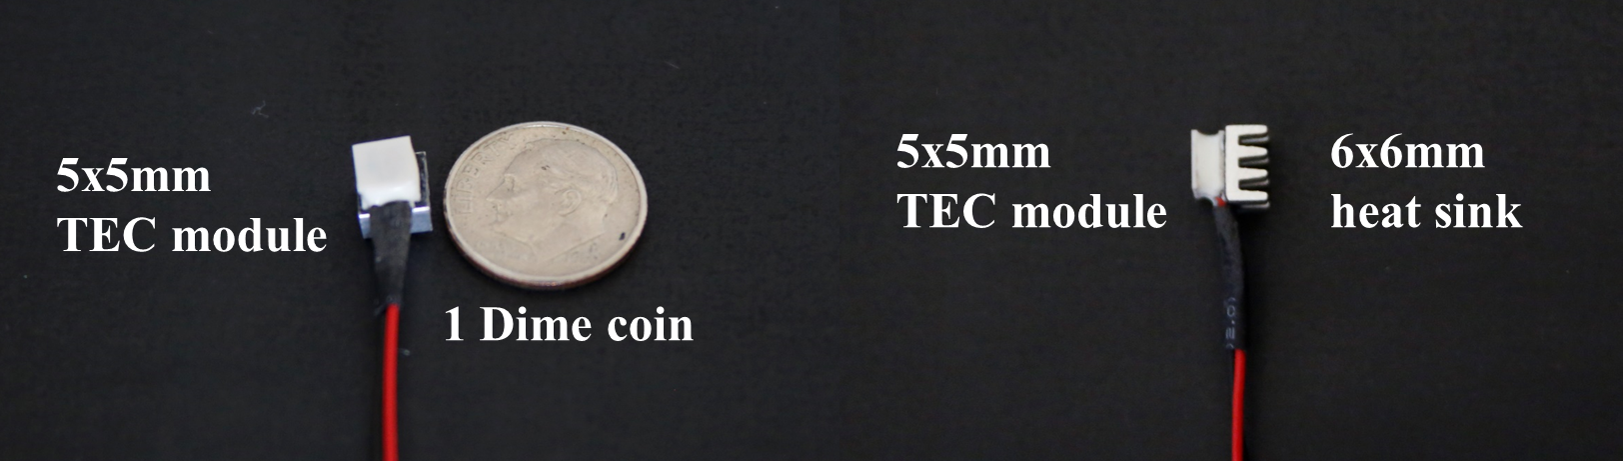
\includegraphics[width=0.8\columnwidth]{img/fig2.png}
  %\subfigure\cite{]{\label{fig:fold2}\includegraphics[width=0.45\textwidth]{images/wo_assembly.png}}
  \caption{TEC Module. Dime for scale.}
  \label{fig:2}
\end{figure}

\begin{figure}[h]
  \centering
  %\subfigure\cite{]{\label{fig:fold1}\includegraphics[width=0.45\textwidth]{images/study_setup.png}}
  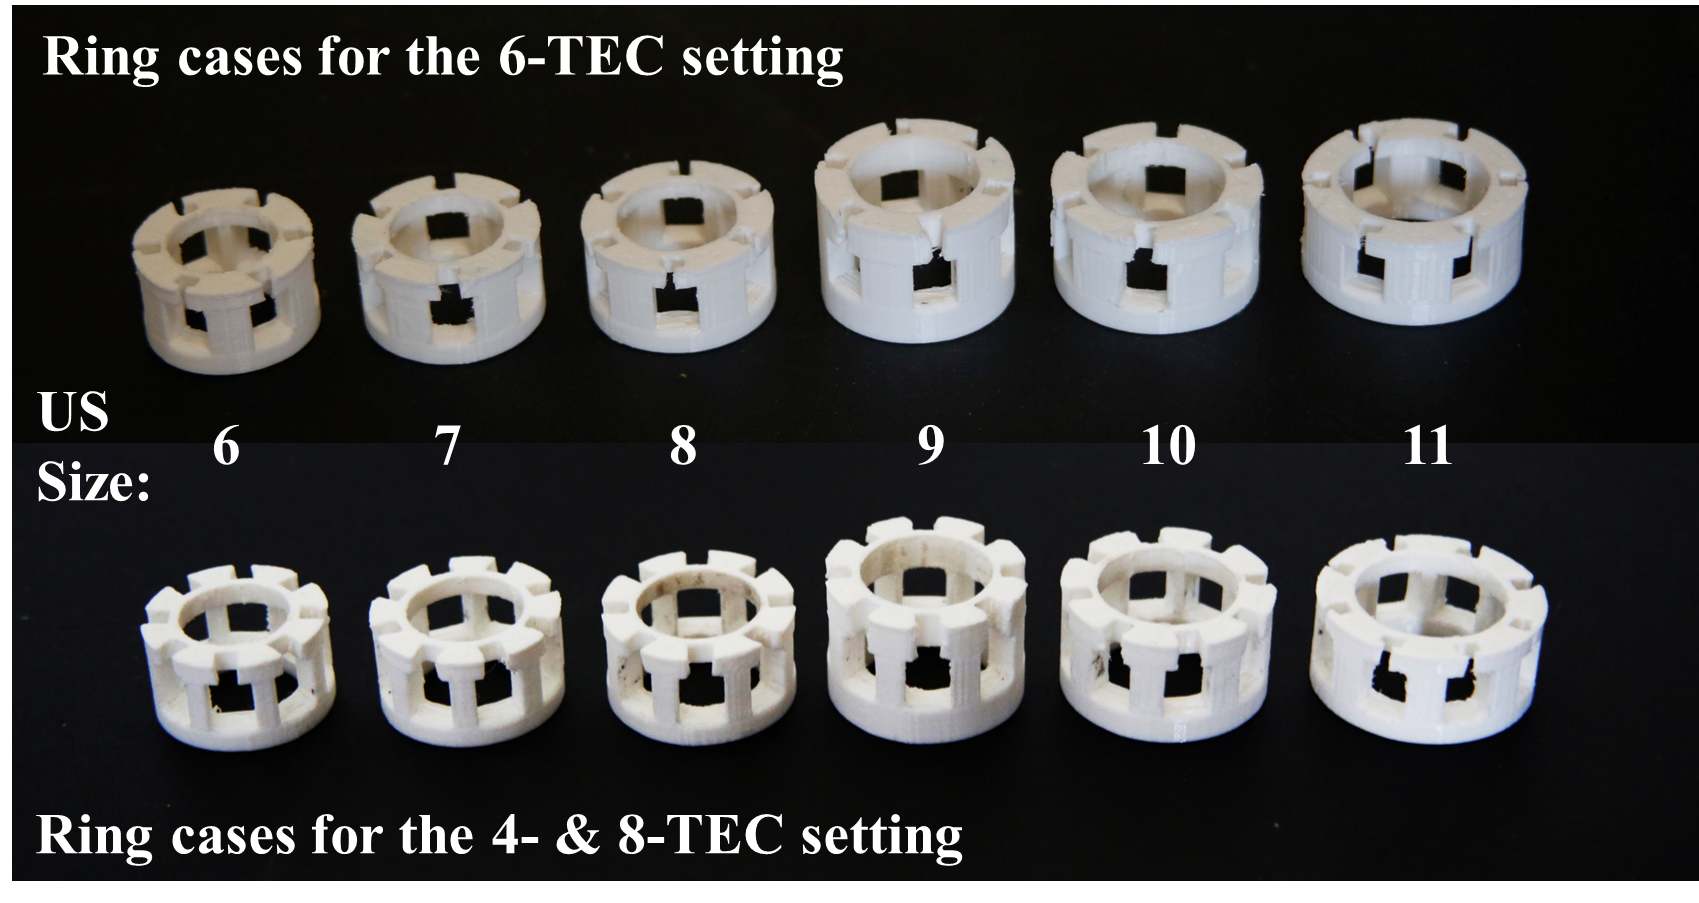
\includegraphics[width=0.8\columnwidth]{img/fig3.png}
  %\subfigure\cite{]{\label{fig:fold2}\includegraphics[width=0.45\textwidth]{images/wo_assembly.png}}
  \caption{Set of rings of different sizes (6 to 11 US sizes) used in this paper.}
  \label{fig:3}
\end{figure}

\begin{figure}[h]
  \centering
  %\subfigure\cite{]{\label{fig:fold1}\includegraphics[width=0.45\textwidth]{images/study_setup.png}}
  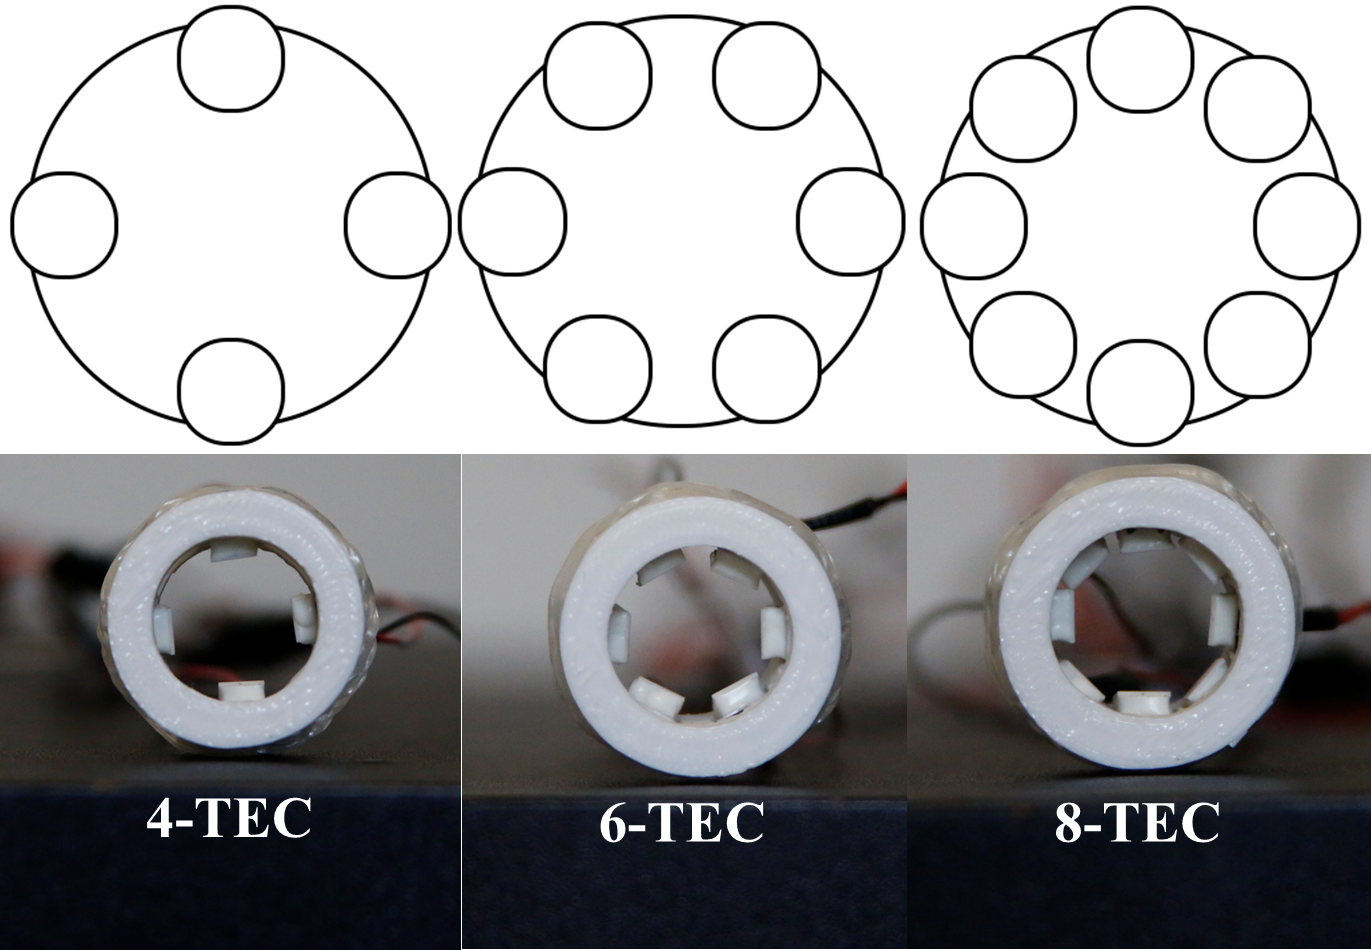
\includegraphics[width=0.8\columnwidth]{img/fig4.png}
  %\subfigure\cite{]{\label{fig:fold2}\includegraphics[width=0.45\textwidth]{images/wo_assembly.png}}
  \caption{Arrangement and assembly of the TEC modules in the three different settings.}
  \label{fig:4}
\end{figure}

\section{Pilot Experiment}
In our pilot experiment, we investigated the resolution of the thermal ring, i.e. the maximum number of discrete points users could perceive around a single finger. We chose three conditions for this experiment: a ring with 4, 6, or 8 TEC elements.

\subsection{Participants}
Nine participants (5 females, 8 right-handed) ranging from 23 to 31 years old (M=26.76, SD=2.78) were recruited from within the university community. The average skin temperature on the finger was 32.6 $^{\circ}$C (SD = 1.342).
%\colorbox{yellow}{Research showed that XX could potentially cause pain.}
Some of our original pool of participants did experience pain when trying the device, which may be due to (a) higher thermal sensitivity at younger ages~\cite{31} and (b) wide variations of thermal sensitivity~\cite{31}.
To ensure the wellbeing of participants and the execution of the experiment, we conducted a 2-minute pre-study session to test the thermal and pain threshold of the recruited participants, and excluded those with overly-sensitive skin.

\subsection{Apparatus}
For this experiment, we designed 12 ring prototypes in sizes ranging from US 6 (diameter of 16.45 mm) to US 11 (diameter of 20.6 mm), as shown in Fig. \ref{fig:3}. Each ring contained 6 or 8 TEC elements on them. For the 4-TEC condition, we only installed 4 TECs in the 8-TEC ring. At the beginning of the experiment, we selected the ring best fit each participant. The rings were worn on the index finger of their non-dominant hand. An iPad Air 2 was used to display the GUI webpage content for training and testing, and allow the participants to select their answers. The GUI webpage was connected to the PC server through a web-socket protocol. All sessions were facilitated by the same experimenter and conducted in a university office with central air-conditioning, maintaining a stable room temperature of 27 $^{\circ}$C.

\subsection{Tasks and Stimuli}
During each test trial, one of the elements would get activated on two temperature levels we chose (hot : + 1 $^{\circ}$C/s and cold : -1 $^{\circ}$C/s) for 3 seconds.
The TECs started the temperature change from the skin temperature of the user.
The participant would then, without looking at their hand, determine on which elements the stimulus happened by selecting the correct element on the iPad Air 2. There was a 15-second  break between trials, to allow the skin naturally return to the resting temperature which was record before the experiment.

\subsection{Procedure}
Participants began the experiment by filling a pre-test questionnaire with demographic information. Their skin temperature on the finger was collected. Before starting, the experimenter helped the participant choose and put on a ring that would best fit on their finger among the six different sizes. The ring was then put on the finger to reach the positions shown in Fig. \ref{fig:4}.

The experiment was divided into three sections (one for each TEC setting). Each section started with a training block where each stimulus was triggered clockwise sequentially starting from the bottom element for the 4-TEC and the 8-TEC setting, and the left element for the 6-TEC setting. During each stimulus in the training, the iPad Air 2 showed the corresponding location being highlighted in blue for cold stimulus or red for hot stimulus (Fig. \ref{fig:5}b). This was repeated twice. After training, participants completed two test blocks, where stimuli were presented in a randomized order. The selection interface was displayed after each stimulation, and participants selected the stimulated element by tapping on the smaller circle in the web page (Fig. \ref{fig:5}c). After completing each test block, participants filled a post-experimental questionnaire to measure the perceived level of difficulty and comfort using a 7-point likert scale (1 - not difficult /comfortable at all, 7 - extremely difficult/comfortable).


\begin{figure}[tp]
  \centering
  %\subfigure\cite{]{\label{fig:fold1}\includegraphics[width=0.45\textwidth]{images/study_setup.png}}
  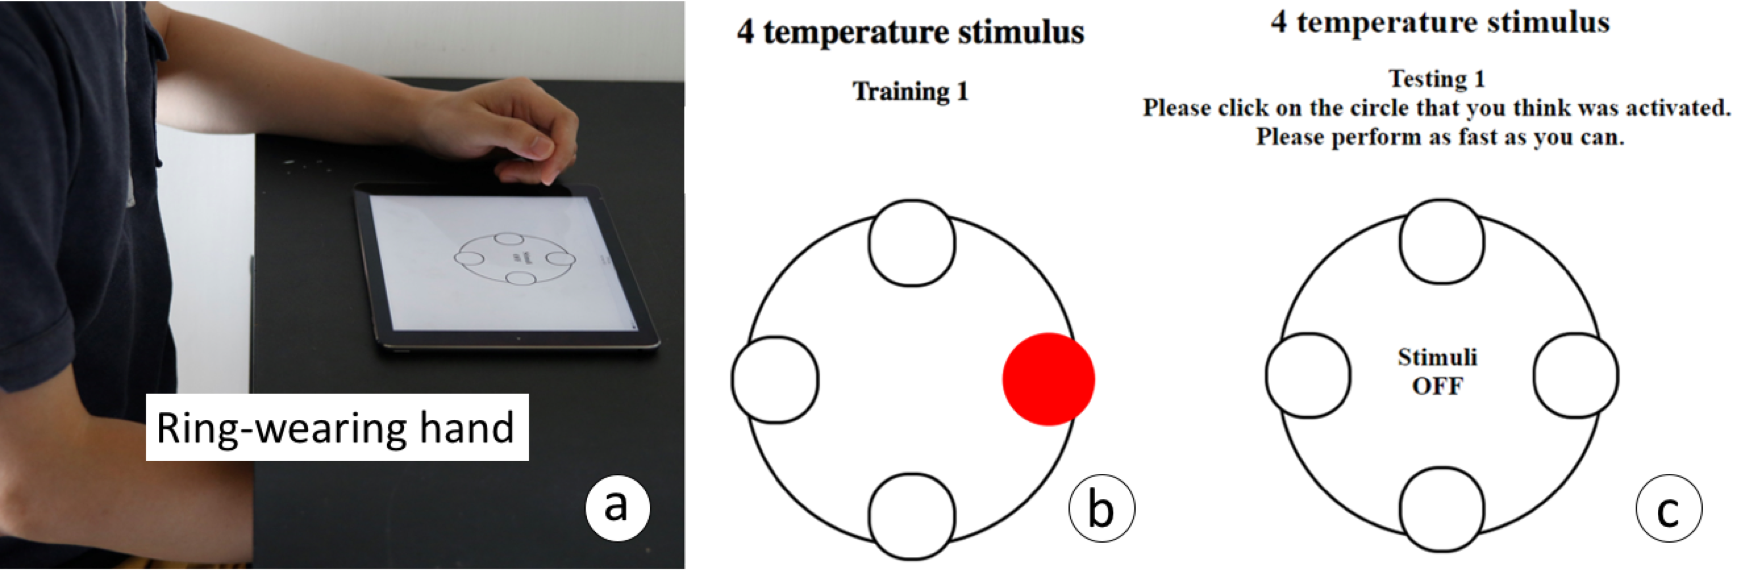
\includegraphics[width=0.8\columnwidth]{img/fig5.png}
  %\subfigure\cite{]{\label{fig:fold2}\includegraphics[width=0.45\textwidth]{images/wo_assembly.png}}
  \caption{(a) Experiment setup; (b) Training Interface for the 4-TEC setting; (c) Testing Interface for the 4-TEC setting.}
  \label{fig:5}
\end{figure}

\subsection{Experiment Design}
A $3 \times 2$ within-subject design was used with two independent variables: number of TECs (4, 6, 8) and temperature change {cold (-1 $^{\circ}$C/s), hot (+1 $^{\circ}$C/s)}. The number of TECs was counterbalanced using Latin Square and temperature was randomized within blocks. We measured two dependent variables: element accuracy and response time (i.e. time to complete a trial after the stimulation). A trial was considered successful when the participant was able to identify the correct element that was activated. Participants could take voluntary breaks between blocks.

Each participant performed the experiment in one sitting (Fig. \ref{fig:5}a), placing his/her ring-wearing hand on the keyboard drawer of the table, thus he/she couldn't see the ring. The experiment lasted for around 70 minutes. In total, each participant did a total of 3 conditions (number of elements) $\times$ 2 temperatures $\times$ [1 training block + 2 test blocks] $\times$ (4+6+8) stimuli = 216 trials.


\subsection{Results}
A repeated measures ANOVA test was conducted for the two dependent variables: the accuracy of element identification and the response time.

\subsubsection{Accuracy of Element Identification}
The accuracy of element identification was significantly affected by the number of TECs ($F_{2,16} = 77.45$, $p < 0.001$, $\eta_p^2 = 0.906$) and the direction of temperature change ($F_{1,8} = 21.34$, $p < 0.01$, $\eta_p^2 = 0.727$).
There was no significant difference between two blocks in terms of accuracy.
A post-hoc Tukey HSD Test showed the accuracy of element identification in the 4-TEC setting (89.9\%) was significantly higher than the accuracy in the 6-TEC setting (73.8\%, $p < 0.0005$), which was significantly higher than the accuracy in the 8-TEC setting (52.7\%, $p < 0.0005$). The accuracy of element identification with cold stimulation (78.7\%) was significantly higher than the accuracy with hot stimulation (65.6\%, $p < 0.005$).

There was no significant interaction effect among the block, the number of TECs, and the direction and temperature change. In all settings, the participants could perceive the stimulated position more accurately with cold stimulation than hot stimulation. More specifically, the participants achieved an accuracy of 97.2\% for cold stimulation and 82.4\% for hot stimulation in the 4-TEC setting (Fig. \ref{fig:6}).

\begin{figure}[tp]
  \centering
  %\subfigure\cite{]{\label{fig:fold1}\includegraphics[width=0.45\textwidth]{images/study_setup.png}}
  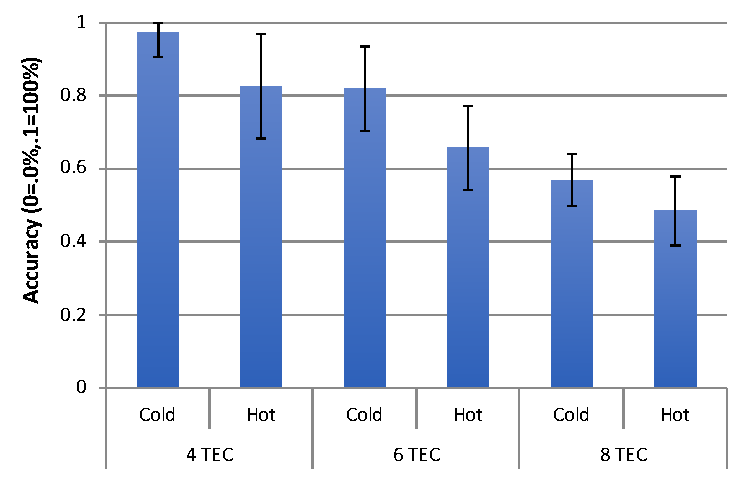
\includegraphics[width=0.7\columnwidth]{img/fig6.pdf}
  %\subfigure\cite{]{\label{fig:fold2}\includegraphics[width=0.45\textwidth]{images/wo_assembly.png}}
  \caption{Accuracy of Element identification for the pilot study. Error bars show .95 confidence intervals.}
  \label{fig:6}
\end{figure}

\subsubsection{Individual Accuracy in 4-TEC setting}
The 4-TEC setting afforded the highest accuracy of element identification. To compare the accuracy of each individual TEC (Fig. \ref{fig:7}), we had a new factor, which was the actuator location (top, right, bottom, left).
We ran a repeated measures ANOVA test, and found a significant main effect of TEC location ($F_{3,24} = 7.53$, $p < 0.005$, $\eta_p^2 = 0.485$) on the accuracy, while there was no significant difference between the two sequential blocks.
More specially, a pair-wise comparison showed that the average accuracy of perceiving the top TEC (97.2\%) was significantly higher than the accuracy of the bottom TEC (80.6\%, $p < 0.05$).
There was no significant difference between the average accuracy of the top TEC and the average accuracy of the left or right TEC (left: 88.9\%, right: 88.9\%).

The direction of temperature change also placed a significant effect on the accuracy ($F_{1,8} = 11.13$, $p < 0.05$, $\eta_p^2 = 0.582$).
A post-hoc pair-wise comparison showed that the average accuracy of identifying the positions of cold stimulus was significantly higher than the the accuracy of hot stimulus ($p < 0.05$).
In addition, there was a significant interaction effect between the TEC position and the direction of temperature change. More specifically, a post-hoc pair-wise comparison revealed that the accuracy of identifying the top TEC was significantly higher than that of the right ($p < 0.05$), the left ($p < 0.05$), and the bottom ($p < 0.05$) TECs with the hot stimulus, while there was no significant difference among the four positions with the cool stimulus.

\begin{figure}[h]
  \centering
  %\subfigure\cite{]{\label{fig:fold1}\includegraphics[width=0.45\textwidth]{images/study_setup.png}}
  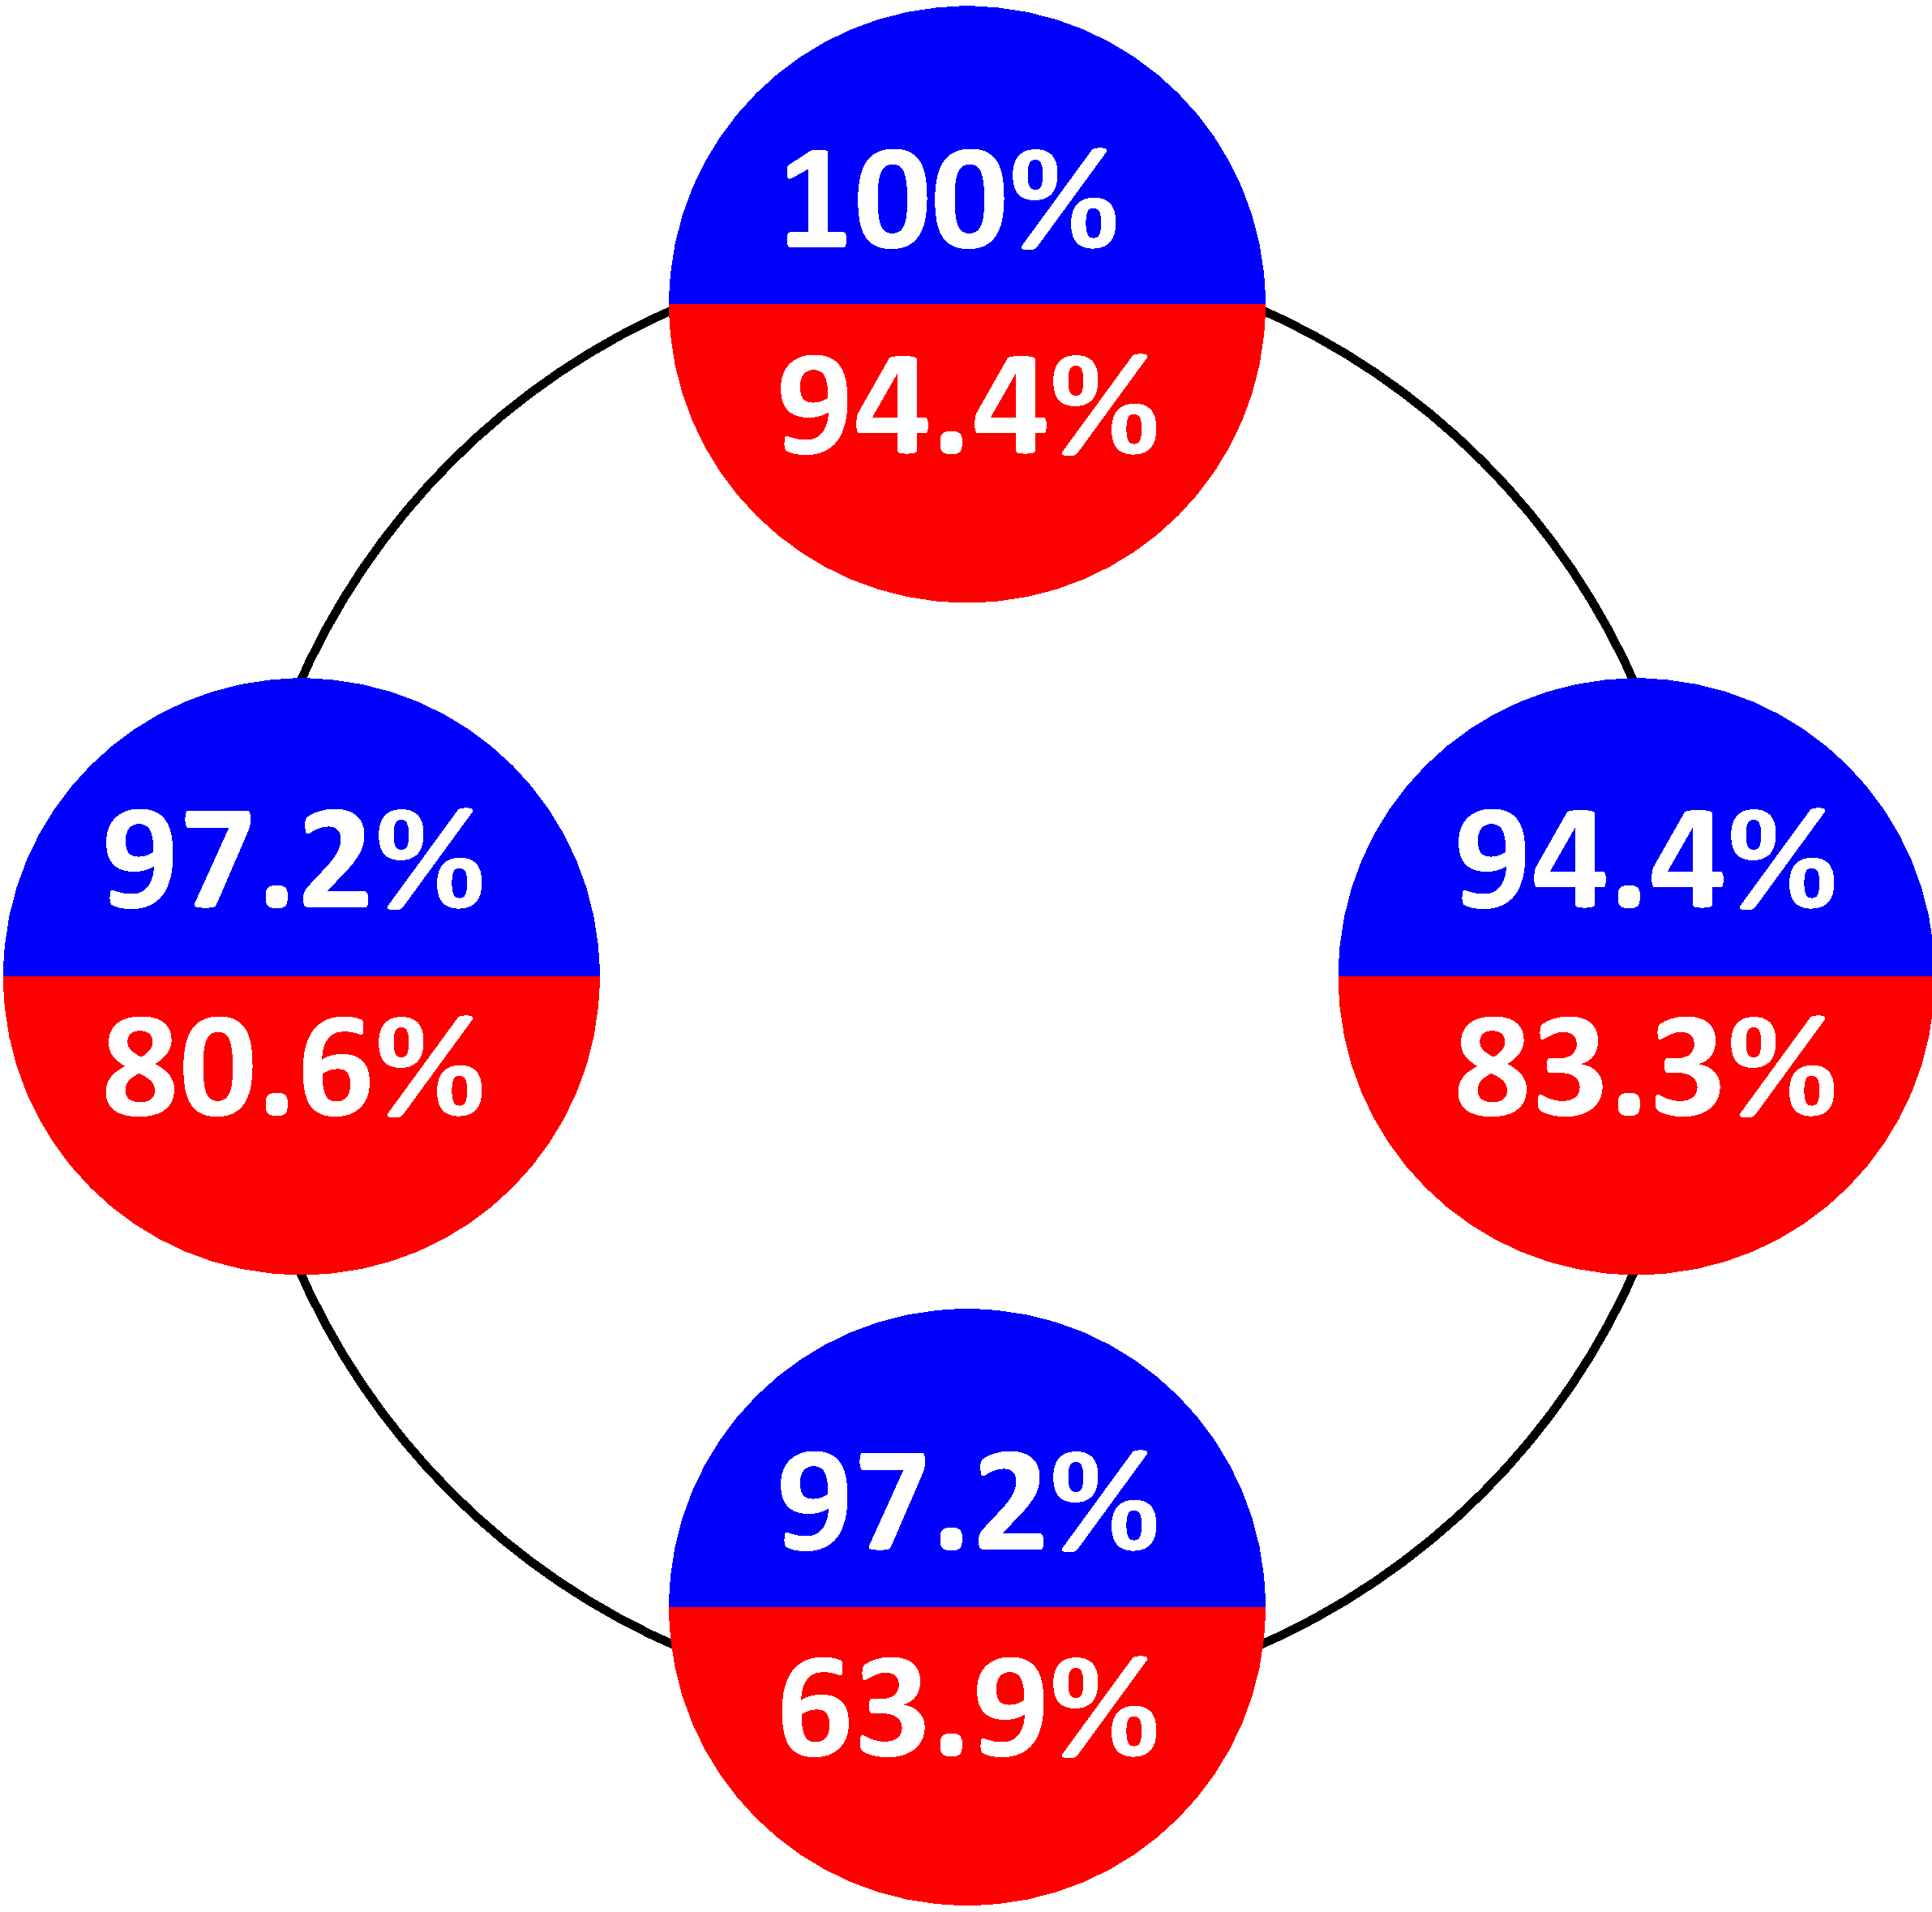
\includegraphics[width=0.4\columnwidth]{img/fig7.pdf}
  %\subfigure\cite{]{\label{fig:fold2}\includegraphics[width=0.45\textwidth]{images/wo_assembly.png}}
  \caption{Accuracy of Individual Element Identification for the 4-TEC setting. Blue: cold stimulation, Red: hot stimulation.}
  \label{fig:7}
\end{figure}

\subsubsection{Response Time}
Response times are summarized in Fig. \ref{fig:8}. Similarly to the accuracy of element identification, a repeated measures ANOVA showed the number of TECs ($F_{2,16} = 78.42$, $p < 0.0005$, $\eta_p^2 = 0.607$) and the direction of temperature change ($F_{1,8} = 20.32$, $p < 0.0001$, $\eta_p^2 = 0.346$) had significant effect on the average response time on one trial.
A post-hoc pair-wise comparison showed that there was no significant difference between the time spent by the participants in the 4-TEC setting (3.37 s) and 6-TEC setting (3.54 s), and the participants performed significantly faster in either of these two conditions than the 8-TEC setting (4.14 s, $p < 0.05$).
The average response time was significantly shorter with cold stimulation than hot stimulation (3.0 s vs. 4.27 s, $p < 0.005$).

\begin{figure}[tp]
  \centering
  %\subfigure\cite{]{\label{fig:fold1}\includegraphics[width=0.45\textwidth]{images/study_setup.png}}
  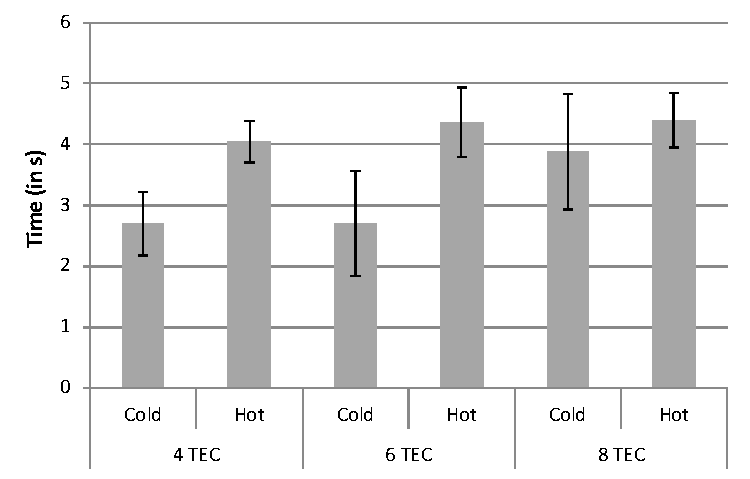
\includegraphics[width=0.7\columnwidth]{img/fig8.pdf}
  %\subfigure\cite{]{\label{fig:fold2}\includegraphics[width=0.45\textwidth]{images/wo_assembly.png}}
  \caption{Response Time for the pilot study. Error bars show .95 confidence intervals.}
  \label{fig:8}
\end{figure}

There was no significant interaction effect of the two independent factors (number of TECs and temperature change) on the average response time on one trial.
In both the 4-TEC and 6-TEC settings, participants performed significantly faster with cold stimulation than hot stimulation (4-TEC: 2.70 s vs. 4.05 s, $p < 0.05$; 6-TEC: 2.70 s vs. 4.36 s). There was no significant difference between the average response time with cold stimulation and hot stimulation in the 8-TEC setting (3.88 s vs. 4.40 s).

\subsection{Discussion}
A significant observation of the pilot study is that participants found it easier to precisely locate a cold stimulation compared to a hot one. This result is in line with previous research on other body locations \cite{10}. Additionally, response time was around 1.2 s faster for cold sensation compared to hot. A direct application of these results point to using a cold temperature change to convey information where correct location perception is crucial, for example, in a navigation scenario where each TEC encodes a direction.

In terms of ring design, our results suggest that participants are able to discriminate up to four locations on the smart ring with good average accuracy (89.9\%). One-way ANOVA on the post-study questionnaire showed a significant effect of the number of TECs on the perceived difficulty of stimulation identification ($F_{2, 51} = 21.59$, $p < 0.005$, $\eta_p^2 = 0.458$).
The post-hoc Tuckey HSD test suggested that the perceived difficulty of stimulation identification for the 4-TEC setting (M = 2.4, SD = 1.4) and the 6-TEC setting (M = 3.2, SD = 1.0) were significantly lower than those the 8-TEC setting (M = 4.8, SD = 1.3, all $p<0.05$). There was no significant difference between the perceived difficulty of the 4-TEC setting and the 6-TEC setting. In addition, the perceived comfort of the 4-TEC setting (M = 5.5, SD = 1.1) was slightly but not significantly higher than those of the 6-TEC setting (M = 5.3, SD = 1.1) and the 8-TEC setting (M = 4.9, SD = 1.2, all $p>0.05$).
By focusing on each individual actuator on the ring, we also found that it was less accurate to perceive a stimulus on the bottom actuator.
Previous work~\cite{31} suggests that thermal sensitivity does not greatly vary across most body parts, excluding the most sensitive ones (head).
However, more recent work from Machado et al.~\cite{Machado2008} suggests that the dorsal part of the hand and fingers (i.e. top location) produces more sweat compared to the palmar part (i.e. bottom location).
While the thermal sensitivity vs. sweat secretion relation is not explicit, the lower performances of our bottom spot, specifically when exposed to hot stimulation, seems to corroborate these previous results.
Therefore, potential spatial thermal patterns may want to make use mostly of the top, right, and left TECs.

\section{Pattern Generation}
Our pilot study confirmed that users can reliably perceive individual thermal stimulation with the 4-TEC setting. To gain a deeper understanding on the affordance and the expressiveness of the 4-TEC setting, we designed new spatial thermal patterns by combining a pair of neighboring or opposite TECs.
Although early studies \cite{26,27,31} on thermal localization showed that radiation-based non-contact heat was error-prone in localization due to the phenomenon of spatial thermal summation, later research suggested on-skin thermal stimuli through small thermal-haptic devices could improve the spatial acuity for tactile stimulation \cite{28}.
In addition, we hypothesised that the change of the thermal intensity caused by the spatial summation could provide hints and assist users to identify different patterns.

In line with previous literature on spatiotemporal vibrotactile patterns~\cite{Alvina2015,Semfeel}, our primary goal is to design a set of patterns that can be easily recognized and convey information quickly. To ensure better recognizability, we decided to use many dimensions with reduced set of values for each instead of fewer dimensions with larger set of values, in order to leverage chunking~\cite{Miller1956}.
A secondary goal is to potentially simple mappings between patterns and applications/commands.

The set of available dimension for vibrotactile pattern includes frequency, amplitude, waveform, duration, rhythm and spatial location~\cite{Brown2005,Chan2008,MacLean2008}. Alvina et al.~\cite{Alvina2015} show that precisely locating a vibrotactile sensation may be problematic and propose a simple binary dimension instead of spatial location which is whether two consecutive pulses happen on the same motor.
MacLean \& Enriques investigated similar dimensions for force feedback.
Thermal feedback is a bit more limited, due to its different nature: a TEC will still remain either hot or cold after being turned off, and that kind of latency makes it hard to work with \textbf{rhythm} or \textbf{waveform}.
Similarly, \textbf{amplitude}, which can be seen as the temperature change rate may induce pain, we thus chose a single value for it.

In order to design our patterns, we considered the following dimensions:
\begin{itemize}
\item Temperature Direction \{ Hot, Cold \}
\item Location \{ Top, Right, Left, Bottom \}
\item Grouping Strategy \{ Neighbors, Opposite \} (for patterns involving two TECs)
\item Temperature Change \{1$^\circ$C/sec\} (controlled)
\item Temporality \{Simultaneous\} (for patterns involving two TECs, controlled)
\end{itemize}

We did not consider more complex spatiotemporal patterns, based on recommendations from Gallace et al.~\cite{Gallace2007} who suggested that participants may recognize simple shapes such as lines (by activating two actuators similar to two points), but only experts may detect more complex shapes. This also allows us to keep the patterns short duration-wise.

Carcedo et al.~\cite{1} investigated the Temporality dimension and advocated to use a sequential temporality (i.e. sensors are not activated simultaneously), but initial testing with TECs did not show any drop of accuracy, allowing us to shorten the patterns by setting the Temporality to simultaneous.

The grouping strategies were tested in two different experiments, as to minimize to keep the number of varying dimensions close to MacLean's~\cite{MacLean2008} recommendations, and, as results will show, to maximize recognizability.

In order to investigate the mapping between patterns and commands, we ran a design workshop. MacLean~\cite{MacLean2008} presented guidelines for haptic icons. While we use different dimensions, we aim to design a set that can be easily mapped, at hopefully a low cognitive cost.
The use of a spatial dimension allows us to create representational icons. For example, leveraging the similarities between cardinal points and our 4 TECs layout allows us to create a simple pattern set for navigation (e.g. activating the Left TECs for Left turn/West, or both Top/Left for North-West). Temperature can also be mapped with emotions~\cite{35,37}, providing another option for simple mapping: a hot stimulus could be used to encode a positive meaning, or the priority of an event.

Finally, it is important to note that we did not consider multimodal icons, as investigated by previous work~\cite{Chan2008}, as we wanted to specifically focus on thermal feedback. However, we do see a strong potential for multimodal icons combining thermal feedback and light, vibration or force feedback.

In our design, each element in a neighboring or opposite pair could be triggered in three thermal levels: hot, neutral, and cold. Therefore, there were eight thermal patterns for each pair. Fig. \ref{fig:9} shows the  patterns on the neighboring pairs (i.e., Top+Left, Top+Right, Bottom+Left, and Bottom+Right). Fig.~\ref{fig:12} shows the patterns on the Top+Bottom and the Left+Right opposite pairs. To facilitate the data analysis, we coded the TEC elements in the 4-TEC setting with the following scheme: bottom - B, left - L, top - T, right - R. The directions of temperature change were coded as: +1 $^{\circ}$C/s - h, -1 $^{\circ}$C/s - c. For example, the pattern ThRc indicates that the top TEC is triggered with +1 $^{\circ}$C/s, and the right TEC is triggered with -1 $^{\circ}$C/s. As indicated by the pilot study, the heat stimulation at the bottom TEC yielded the lowest identification accuracy, so we excluded the patterns involving the heat stimulation at the bottom TEC (i.e., BhLh, BhLc, BhRh, BhRc, ThBh, and TcBh).


\begin{figure}[tp]
  \centering
  %\subfigure\cite{]{\label{fig:fold1}\includegraphics[width=0.45\textwidth]{images/study_setup.png}}
  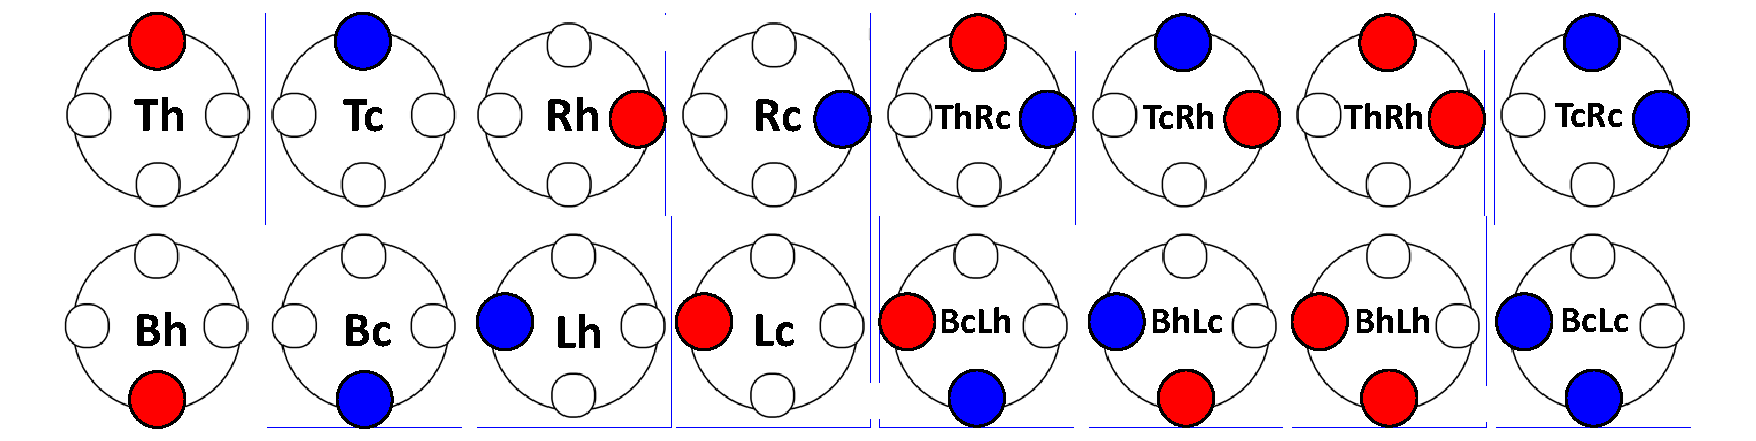
\includegraphics[width=0.9\columnwidth]{img/fig9.pdf}
  %\subfigure\cite{]{\label{fig:fold2}\includegraphics[width=0.45\textwidth]{images/wo_assembly.png}}
  \caption{Patterns (with names) for neighboring TECs, applied on the Top+Right and the Bottom+Left TECs. Red: hot; Blue: cold; White: neutral.}
  \label{fig:9}
\end{figure}

Our pilot experiment showed that the participants perceived the cold stimulus 1.2 seconds faster than the hot stimulus. Therefore, while implementing the thermal patterns that contain both hot and cold stimulations (Fig.~\ref{fig:9}: ThRc, TcRh, \& BcLh; Fig.~\ref{fig:12}: ThBc, LcRh, \& LhRc), we placed a 1.2-second gap between the hot and the cold stimulation, meaning the cold stimulation was triggered 1.2 seconds after the hot stimulation, to provide a simultaneous sensation of hot and cold.

\section{Experiment 1: Temperature Changes on Neighboring TECs}
In this experiment, we investigated if participants could recognize temperature changes on neighboring TECs.

\subsection{Participants}
We applied the same recruitment strategy as the pilot study. Twelve participants (7 females, all right-handed) ranging from 18 to 31 years old (M=26.3, SD=3.52) were recruited from within the university community. The average skin temperature on the finger was 32.5 $^{\circ}$C (SD = 1.52).

\subsection{Apparatus}
We used the same apparatus as in the pilot experiment: 6 ring prototypes (US size 6 to 11) with 4 TECs on them. The rings were worn on the index finger of the participants' non-dominant hands. An iPad Air 2 was used for the participants to select their answers.

\subsection{Tasks and Stimuli}
During a single trial, two TECs were activated at one of the two temperature levels (cold, and hot). The participant had to accurately recognize the temperature level of each TEC. We conducted the experiment with all possible neighboring pairs of TECs as shown in Fig. \ref{fig:9}.


\subsection{Procedure}
Similar to the pilot study, participants began the experiment by filling a pre-questionnaire with demographic information, and the experimenter would helped the participant to put on the ring that best fit their finger.

The experiment was divided into two blocks: one training block and one testing block. In a given block, the twelve patterns were presented three times in a randomized order. In the training block, the participant was told which pattern was just triggered with the visual patterns in Fig. \ref{fig:9} shown on the iPad Air 2, while in the testing block, they had to recognize the pattern by selecting the stimulated elements and temperatures. Fig. \ref{fig:10} shows the selection interface we used in the test block. When the stimulation was off, a pair of red and blue circle buttons was shown next to each spot. The participant needed to make their selection by tapping on the buttons, and tapping the ``Next'' button to trigger a new stimulation. After completing the two blocks, participants filled out a post-experimental questionnaire to measure the perceived level of difficulty and comfort of detecting the thermal patterns using a 7-point likert scale, following the similar scheme in the pilot study. The participants also needed to elicit potential applications for the thermal patterns.

\begin{figure}[h]
  \centering
  %\subfigure\cite{]{\label{fig:fold1}\includegraphics[width=0.45\textwidth]{images/study_setup.png}}
  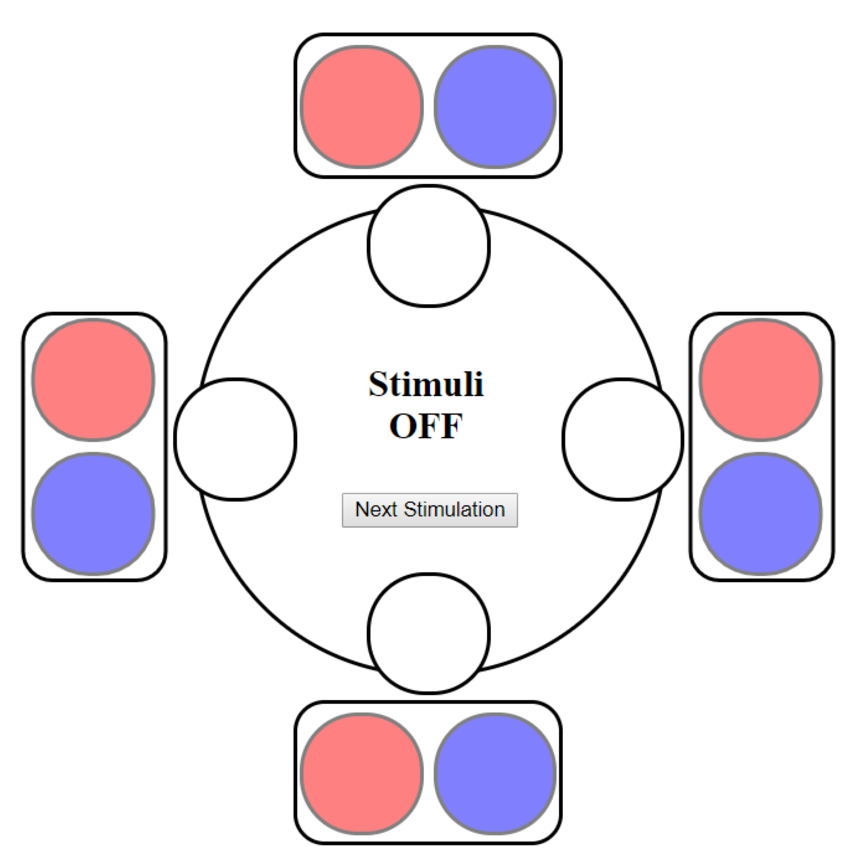
\includegraphics[width=0.5\columnwidth]{img/fig10.pdf}
  %\subfigure\cite{]{\label{fig:fold2}\includegraphics[width=0.45\textwidth]{images/wo_assembly.png}}
  \caption{Selection interface for Experiment 1 \& 2.}
  \label{fig:10}
\end{figure}

\subsection{Experiment Design}
A within-subject design was used with one independent variable: pattern. We measured two dependent variables: accuracy and response time. A trial was considered successful when the participant was able to identify the correct location and temperature level for both TECs. There was a 25-second break between two trials, for the skin to naturally return to the resting temperature.

Each participant performed the experiment in one sitting, including breaks. The experiment lasted for around 45 minutes. In total, each participant did a total of 12 patterns $\times$ [1 training blocks + 1 test block] $\times$ 3 repetitions = 72 trials.

\subsection{Results}
The repeated measure ANOVA showed that the type of the neighboring thermal pattern significantly affected the identification accuracy ($F_{11,121} = 5.42$, $p < 0.0005$, $\eta_p^2 = 0.33$), but had no significant effect on the average time (overall average time = 4.14s, SD = 0.19).
Generally, the participants could identify the patterns that combined two cold stimulations more accurately than the patterns with two hot stimulations and those with a mix of hot and cold stimulations.
A post-hoc pair-wise comparison on the identification accuracy revealed that TcRc (Mean = 86.1\%) yielded significantly higher accuracy than TcLh ($p < 0.0005$, Mean = 19.4\%), BcLh ($p < 0.0005$, Mean = 38.9\%), ThLh ($p < 0.005$, Mean = 44.4\%), ThRh \& TcRh ($p < 0.05$, Mean = 52.8\%), ThLc ($p < 0.05$, Mean = 58.3\%), and ThLc \& BcRh ($p < 0.05$, Mean = 44.4\%).
TcRc was also marginally more accurate than ThRc ($p = 0.067$, Mean = 67\%). BcRc (Mean = 83.3\%) was significantly more accurate than TcLh ($p < 0.0005$), BcLh ($p < 0.05$), ThLh ($p < 0.05$), ThRh ($p < 0.05$), ThLc ($p < 0.05$), and BcRh ($p < 0.05$). TcLc (Mean = 80.6\%) was significantly more accurate than TcLh ($p < 0.0005$), BcLh ($p < 0.05$), TcRh ($p < 0.05$), ThLc ($p < 0.05$), and ThLh ($p < 0.05$).
The only cold-combination pattern with an average accuracy lower than 80\% was BcLc (75.0\%), and it was significantly more accurate than TcLh ($p < 0.0005$), and marginally more accurate than BcLh ($p = 0.053$), ThLh ($p = 0.059$), TcRh ($p = 0.071$), and ThLc ($p = 0.082$).
Fig.~\ref{fig:11} shows the descriptive result of the average identification accuracy and the confusion table for the neighboring patterns.

\begin{figure}[tp]
  \centering
  %\subfigure\cite{]{\label{fig:fold1}\includegraphics[width=0.45\textwidth]{images/study_setup.png}}
  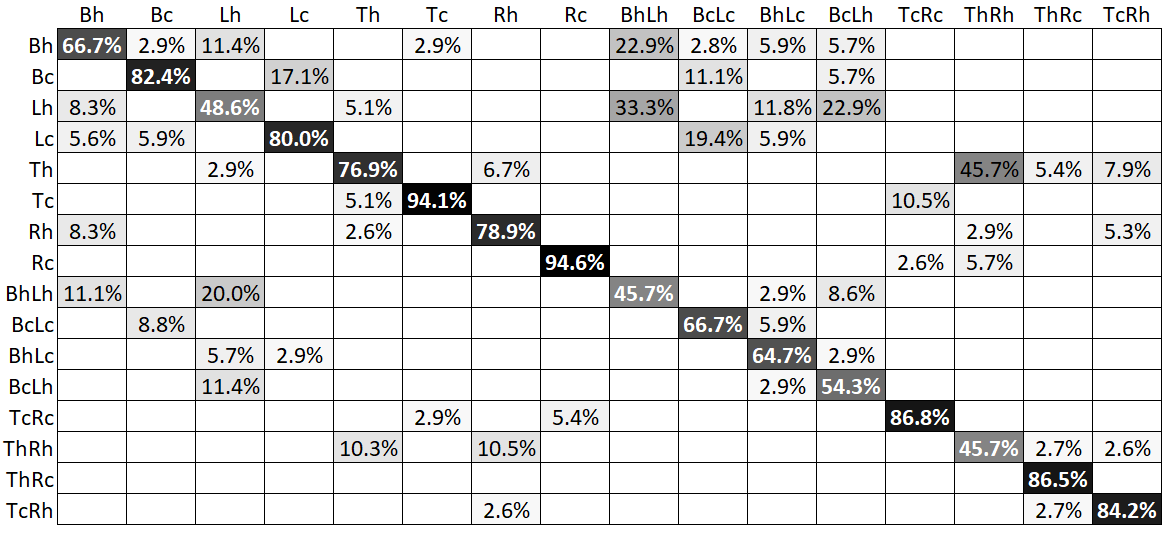
\includegraphics[width=0.9\columnwidth]{img/fig11.png}
  %\subfigure\cite{]{\label{fig:fold2}\includegraphics[width=0.45\textwidth]{images/wo_assembly.png}}
  \caption{Confusion table for the neighboring thermal patterns. Columns represent stimulated pattern and rows the participants' input.}
  \label{fig:11}
\end{figure}

\subsection{Summary}
We noted that 3 out of 12 neighboring patterns had over 80\% accuracy: TcRc, BcRc, and TcLc. Additionally, BcLc achieved 75\% accuracy. All these patterns combined two cold stimulations. This set of patterns confirms that participants had trouble precisely locating hot sensations in the neighboring patterns, either combining two neighboring hot TECs or mixing one hot TEC and one neighboring cold TEC. This could be explained with the previous research which revealed that the spatial summation of thermal sensation placed less effect for cold stimulation than hot stimulation~\cite{43}.

\section{Experiment 2: Temperature Changes on Opposite TECs}
We believe that our proposed ring design can also be used to compare different quantities, such as the ratings of two shops, which could be encoded using different temperatures for the opposite pair of TECs. We conducted another experiment similar to Experiment 1, which considered opposite TECs instead.

\subsection{Participants}
The same recruitment strategy was applied. Twelve participants (5 females, all right-handed) ranging from 19 to 31 years old (M = 22.3, SD = 3.57) were recruited from within the university community. The average skin temperature on the finger was 33.6$^{\circ}$C (SD = 1.53).

\subsection{Apparatus, Task and Stimuli, Procedure}
We used the exact same apparatus and procedure as Experiment 1. The six patterns are shown in Fig.~\ref{fig:12}.

\begin{figure}[tp]
  \centering
  %\subfigure\cite{]{\label{fig:fold1}\includegraphics[width=0.45\textwidth]{images/study_setup.png}}
  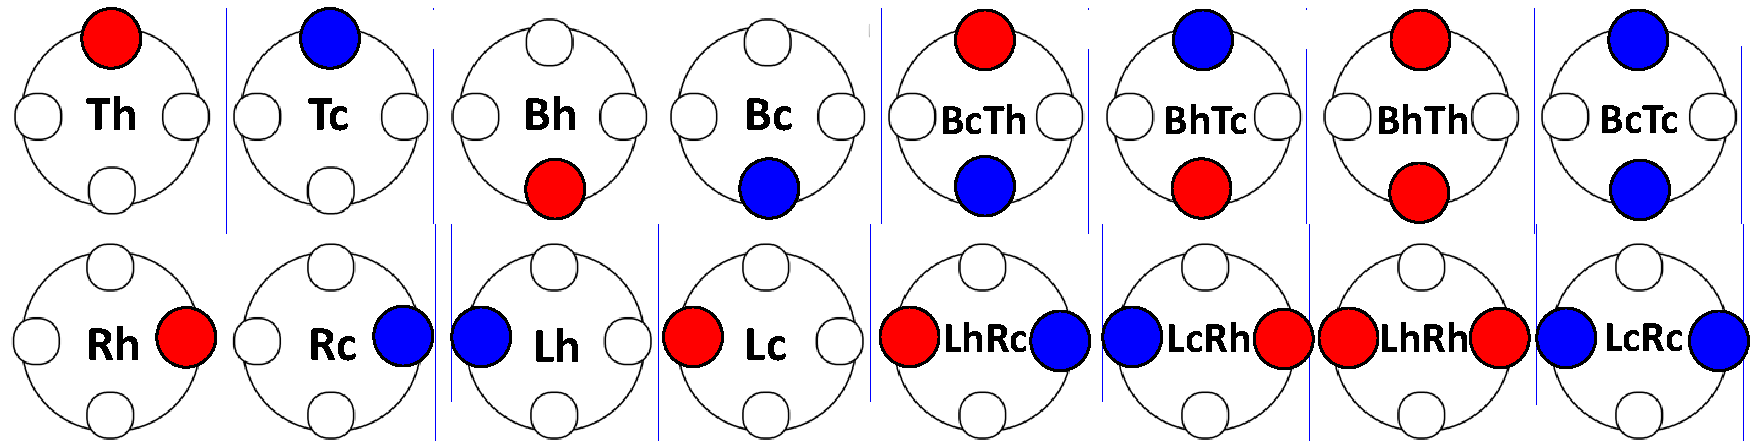
\includegraphics[width=0.9\columnwidth]{img/fig12.pdf}
  %\subfigure\cite{]{\label{fig:fold2}\includegraphics[width=0.45\textwidth]{images/wo_assembly.png}}
  \caption{Patterns (with names) for opposite TECs, applied on the Top+Bottom and the Left+Right TECs. Red: hot; Blue: cold.}
  \label{fig:12}
\end{figure}

\subsection{Experiment Design}
The design of Experiment 2 was similar to Experiment 1. Our only independent variable was the TEC pattern, which was randomized within blocks. We measured location accuracy, temperature accuracy, and the response time. A trial was considered successful when the participant was able to identify the correct temperature level for both TECs. Each participant performed the experiment in one sitting, including breaks. The experiment lasted for around 30 minutes. In total, each participant did a total of 6 patterns $\times$ [1 training block + 1 test blocks] $\times$ 3 repetitions = 36 trials.


\subsection{Results}
Similar to the neighboring patterns, repeated measures ANOVA showed that there was a significant difference among these opposite thermal patterns in terms of the identification accuracy ($F_{5, 55} = 5.18$, $p < 0.01$, $\eta_p^2 = 0.330$).
 Fig.~\ref{fig:13} illustrates the confusion table for the opposite thermal patterns.
 The accuracy for LhRh (61.1\%) was significantly lower than TcBc (91.7\%, $p < 0.05$), ThBc (91.7\%, $p < 0.05$), LcRc (91.7\%, $p < 0.05$), LhRc (83.3\%, $p < 0.05$), and LcRh (83.3\%, $p < 0.05$).

 Besides the identification accuracy, repeated measures ANOVA suggested that the factor of pattern placed a significant effect on the average time for trial completion ($F_{5, 55} = 4.20$, $p < 0.05$, $\eta_p^2 = 0.275$). Post-hoc pairwise comparisons showed that LhRh required significantly longer time (6.02s) for identification than all other patterns ($p < 0.05$, TcBc: 4.53s, LhRc: 4.65s, LcRc: 4.93s, ThBc: 4.99s), except LcRh (5.0s) with which the difference was only marginal ($p = 0.06$).

\begin{figure}[tp]
  \centering
  %\subfigure\cite{]{\label{fig:fold1}\includegraphics[width=0.45\textwidth]{images/study_setup.png}}
  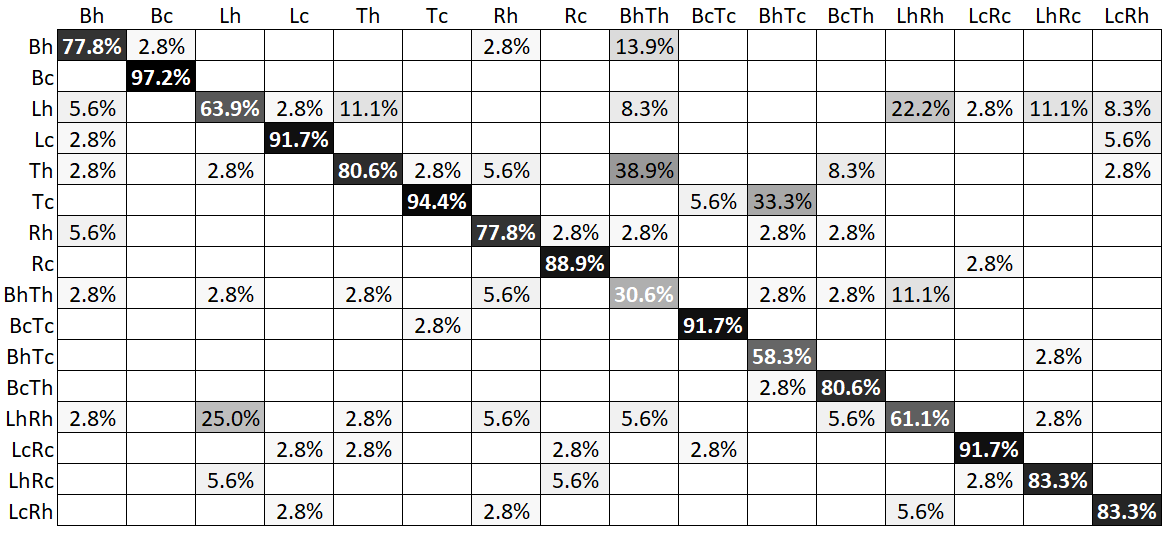
\includegraphics[width=0.9\columnwidth]{img/fig13.png}
  %\subfigure\cite{]{\label{fig:fold2}\includegraphics[width=0.45\textwidth]{images/wo_assembly.png}}
  \caption{Confusion table for the opposite thermal patterns. Columns represent stimulated pattern and rows the participants' input.}
  \label{fig:13}
\end{figure}

\subsection{Discussion}
In terms of accuracy, we found five patterns with 80\% accuracy or more: LcRc, BcTc, BcTh, LhRc, and LcRh. Similar to the former experiment on the neighboring patterns, the patterns involving two cold stimulation (i.e. BcTc and LcRc) resulted in highest accuracy (91.7\%), and LhRh which involved two hot stimulations yielded the lowest accuracy, and the longest identification time. This could also be explained with the effect of spatial thermal summation which confused the participants more with hot stimulation than cold stimulation.

On the other hand, different from the neighboring patterns, the opposite patterns involving the mix of hot and cold stimulations could be identified with accuracy higher than 80\%.
Since the TECs involved were further away from each other compared to neighbors, effects of spatial summation were likely smaller, leading to better overall accuracy.


\section{Selecting and Validating Reliable In-Ring Thermal Patterns}
Our pilot study showed that the participants could identify the single-spot cold TEC significantly better than the hot TEC, and Experiment 1 \& 2 revealed a set of two-spot spatial thermal patterns with the average accuracy above 80\%, including three neighboring patterns and five opposite patterns. However, these patterns were tested separately within their own categories. It is unknown whether users could reliably perceive them when these patterns were grouped together and presented as a whole set of in-ring thermal feedbacks. To answer this question, we conducted three follow-up experiments to validate different group combinations of the selected thermal patterns. These three follow-up experiments adopted the same participant-recruitment strategy, apparatus, procedure, and design as the Experiment 1 \& 2, expect the different group combinations of thermal patterns.

%\section{Validating The Combination of Pattern Groups}
\subsection{Follow-up Experiment 1: Single+Neighbor+Opposite}
We first created a large group of thermal patterns by combining four single-spot cold stimulation (Tc, Bc, Lc, Rc), three neighboring patterns (TcRc, TcLc, BcRc), and five opposite patterns (BcTc, BcTh, LcRc, LhRc, LcRh), and investigated users' identification accuracy and time for each of them. Twelve participants (6 females, all right-handed) ranging from 22 to 30 years old (M = 25.3, SD = 3.27) were recruited from within the university community. The average skin temperature on the finger was 33.4$^{\circ}$C (SD = 1.32). The experiment lasted for around 60 minutes. In total, each participant did a total of 12 patterns $\times$ [1 training block + 1 test blocks] $\times$ 3 repetitions = 72 trials.

%\subsubsection{Results}
The descriptive results and the confusion table, as shown in Fig. XXX, suggested that it was difficult for the participants to reliably perceive these twelve patterns all together in the same group. There were only two patterns with the accuracy above 80\% (i.e., ThBc: 96.7\%, and LcRh: 83.3\%). The confusion table further revealed that the participants tended to confuse the neighboring patterns and the opposite patterns. For example, 30.6\% of TcRc were identified as BcTc, 27.8\% of BcRc were identified as LhRc, 34.2\% of TcBc were identified as TcRc, and 50\% of TcLc were identified as BcTc.
The overall low accuracy may be explained by too many confusing combinations, which combined to spatial summation likely impaired recognition.
%[XXX: how do we explain? Too many confusing items?]

%Accuracy: F(11,121) = 6.03, p < 0.005, $\eta_p^2$ = 0.354
%Time: F(11,121) = 3.43, p < 0.005, $\eta_p^2$ = 0.238

\subsection{Follow-up Experiment 2 \& 3: Single+Neighbor and Single+Opposite}
As the first follow-up experiment suggested that users could not accurately identify the thermal patterns from a large group, it was of our interest to investigate the feasibilty of grouping the single-spot cold stimulations with either the neighboring or the opposite patterns. We first investigated the combination of the single-spot cold stimulations and the neighboring patterns. Twelve participants (6 females, all right-handed) ranging from 22 to 30 years old (M = 24.2, SD = 2.42) were recruited from within the university community. The average skin temperature on the finger was 33.4$^{\circ}$C (SD = 1.26). The experiment lasted for around 30 minutes. In total, each participant did a total of 7 patterns $\times$ [1 training block + 1 test blocks] $\times$ 3 repetitions = 42 trials.  The confusion table in Fig. XXX showed that the participants could identify all seven patterns with the accuracy larger than 80\%. Repeated Measures ANOVA suggested no significance difference among the patterns in terms of accuracy and completion time.

Another twelve participants, 6 females and 6 males, aging from 22 to 32 years old (M = 25.1, SD = 3.22), were recruited for third follow-up experiment to investigate the accuracy and time of identifying the grouped patterns of the single-spot cold stimulations and the opposite patterns. The experiment lasted for around 45 minutes. In total, each participant did a total of 9 patterns $\times$ [1 training block + 1 test blocks] $\times$ 3 repetitions = 54 trials. The confusion table in Fig. XX showed that all these patterns yielded the accuracy above 80\%, similar to the group combination of the single-spot cold stimulations and the neighboring patterns. Repeated Measures ANOVA showed that there was no significant difference among these patterns in terms of the identification accuracy and trial-completion time.
%No significant difference on accuracy. all $>$ 80\%.
%No significant difference on time.

\subsection{Summary of Follow-up Experiments}
XXX
[Lead to the design workshops]

\section{Design Workshops for Mapping In-Ring Spatial Thermal Patterns to Information Representation}
The follow-up experiments suggested that the combined group of single-spot cold stimulations and neighboring/opposite patterns could be identified reliably with the accuracy above 80\%, suggesting the potential usage of these in-ring thermal patterns as thermal icons for information representation. To distill the potential mapping of these thermal patterns (4 single-spot cold stimulations, 3 neighboring patterns, and 5 opposite patterns) and the information in various application scenario, we conducted a series of design workshops, involving six experienced product/interface designers (3 females and 3 males, average age = 34.3 years old).

\subsection{Workshop Procedure}
We conducted three design workshops, each of which involved two designers. Each workshop started with an initial ice-breaking session in which the facilitator introduced the concept of in-ring spatial thermal feedback and the purpose of the workshop. The designers then wore the ring and experienced the thermal patterns which were triggered in randomized order with the visual representations shown on the iPad 2. They could experience any of these thermal patterns at any time during the design workshop. The facilitator then asked the designers to select a subset of the twelve spatial thermal patterns (Figure~\ref{fig:workshop}) for six common application categories that could be potentially benefit from thermal feedback based on previous research [XX]: emotion representation, call/message notification, navigation, artefact properties (e.g., ratings of service), calendar, and game. The facilitator also instructed the designers to follow these design rules: 1) The designer can create the mappings for multiple scenarios within one application category; 2) Each pattern should be used only once within one application scenario; 3) The patterns can be reused across difference scenarios; 4) The single-spot stimulations can be used with the neighboring or opposite patterns within one application scenario; 5) The neighboring and the opposite patterns can not be used within the same scenario; 6) The designers need to write clearly the rationale for every design choice in the given paper form.

There were two design sessions in each workshop. The designers created their own mappings individually in the first session, and discussed with each other to create a new mapping by summarizing the individual mappings in the second session. They can reuse their individual design mappings in the second session. The workshop lasted around 1 hour.

\begin{figure}[tp]
  \centering
  %\subfigure\cite{]{\label{fig:fold1}\includegraphics[width=0.45\textwidth]{images/study_setup.png}}
  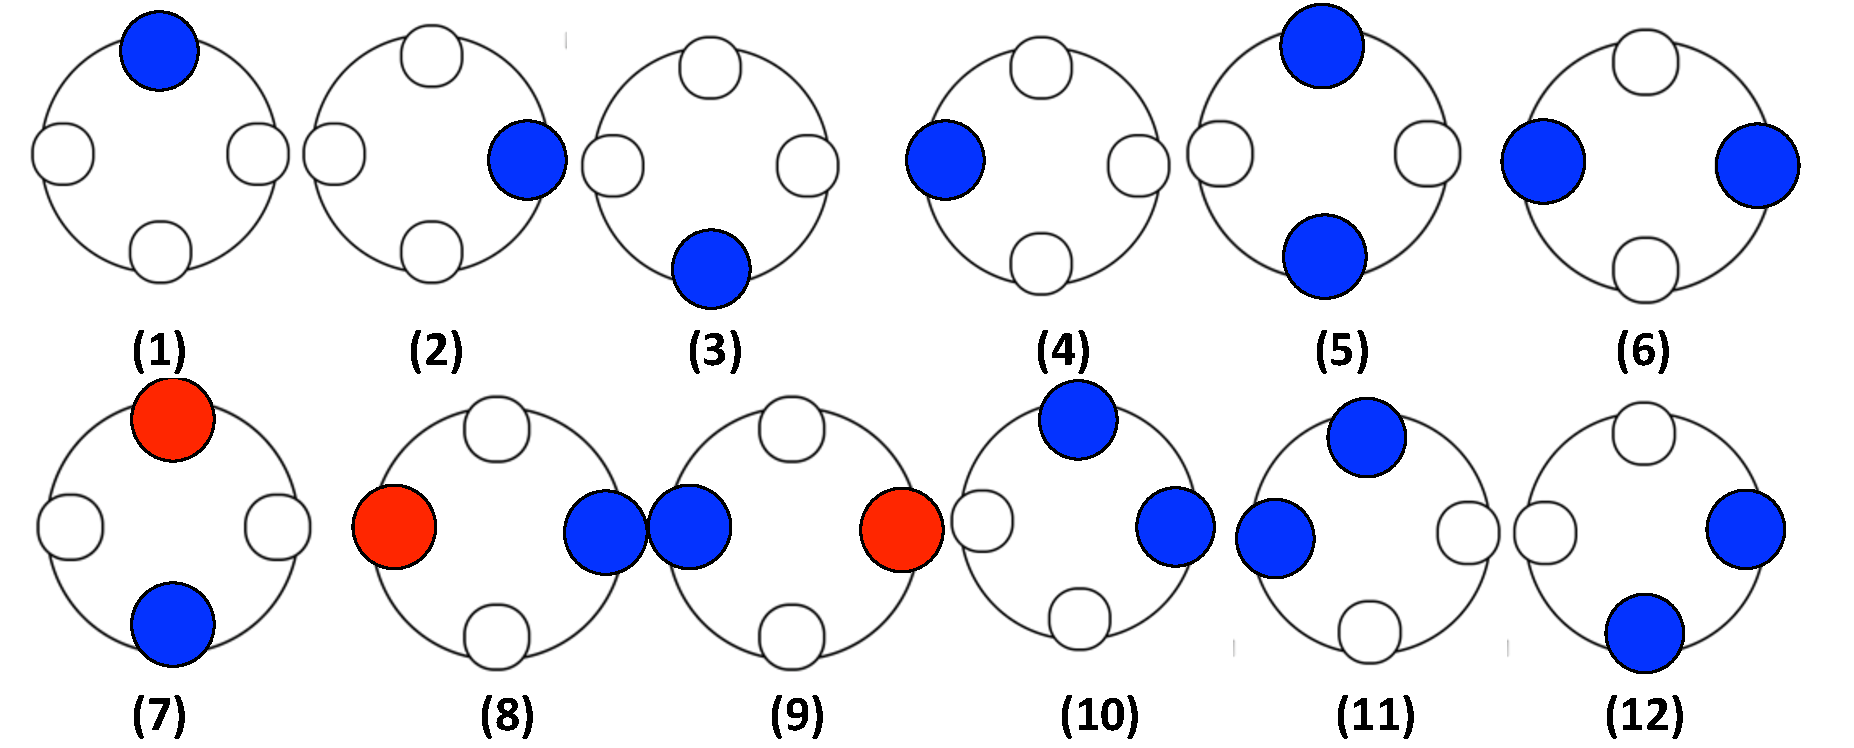
\includegraphics[width=0.9\columnwidth]{img/fig-workshop.pdf}
  %\subfigure\cite{]{\label{fig:fold2}\includegraphics[width=0.45\textwidth]{images/wo_assembly.png}}
  \caption{Set of patterns used during our workshop. The first four involve only 1 TEC (single-spot stimulation, \#1--4), the next five involve 2 opposite TECs (\#5--9) and the last three involve neighboring TECs ((\#10--12))}
  \label{fig:workshop}
\end{figure}

\subsection{Workshop Results}
In total, there were 340 mappings created for 14 thermal patterns and 6 application categories. Considering the three groups of thermal patterns, Pearson Chi-Square Test (${\chi}^2(10, N=340) = 61.78$, $p < 0.001$, Cramer's V = 0.301) revealed that there was a significant relationship between the application category and the usage of the thermal patterns by the designers in the workshop.
\\
\paragraph{Navigation}
More specifically, the largest group of mappings (26.6\%) for the single-spot stimulations were to the scenario of navigation.
69\% of the mappings for the neighboring patterns were about the application of navigation.
All of our participants mapped Patterns 1 (Tc), 2 (Rc) and 4 (Lc) with their respective directions. Four out of six participants also mapped Pattern 3 (Bc) with a South/Go backward direction, while the two other mapped them with respectively Pattern 7 (BcTh) and Pattern 6 (RcLc), with the rationale that going backwards, e.g. making a u-turn needs a stronger warning or less expected pattern compared to the other three directions.
The neighboring patterns (10--12) were also mapped to collateral directions, such front-left and front-right.
These simple mapping while seemingly trivial are also extremely easy to learn as they do represent direction in a clear way.
Another interesting result we found that two designers mapped Pattern 11 (TcRc) to Front-Left and Pattern 12 (BcRc) to Front-Right.
The designers explained that this type of mappings was specifically for driving when users, with the ring worn on their left hands, are grabbing the steering wheel, and their hands are perpendicular to the horizontal ground, so that the right position becomes the top position, with the top becoming left and the bottom becoming right.
This suggests that actually knowing the orientation of the finger would allow us to dynamically change the patterns for specific directions in order to maintain a spatial consistency of directions.
Finally, four participants also used pattern with hot stimulation to notify the user of an emergency, such as an obstacle, tunnel, red traffic light or unexpected traffic.

\paragraph{Incoming Messages and Calls}
Our designers vastly (5/6) preferred single-spot patterns to encode four different categories of contacts (mainly friends, family, work, other).
Similarly to navigation, patterns involving hot stimulation (7--9) were used by four designers as a warning of either an unknown contact calling/messaging, harassing call or an urgent call.
The contrast with the otherwise cold stimulation was thus expected to catch the attention, as well as consistently mapping hot stimulation with emergency or warning.


\paragraph{Emotion and Mood}
We asked our participants to select patterns and map emotion with them.
Interestingly they tended to do so by mapping the position of each TEC to feelings.
For example, positive emotions such as good mood/joy were associated with Pattern 1 (Tc) by four participants.
Similarly, feelings of sadness or angryness were mapped with Pattern 3 (Bc): P3 reported \textit{The bottom position means ``I am feeling down''}.
Other patterns involving the bottom position were also suggested, such as Pattern 12 (BcRc), chosen by two participants for sadness, as well as Pattern 7 (BcTh) suggested for anger by one participant.
Pattern 7 was also used by one participant to notify users that their interlocutor should not be disturbed.
Finally, patterns with hot stimulation were used to convey negative emotions: Pattern 7 and 9 were chosen to express anger (two participants) or sadness (two participants).

\paragraph{Properties of Artefacts}
While being used for presenting artifact properties, all designers agreed that the opposite patterns can be used to compare two different artifacts.
For example, when two restaurants, one on the left and the other on the right, are selected for comparison, the side with a higher temperature indicates a higher rating, and the colder side indicates a lower rating.
Patterns 7, 8 and 9 (hot stimulation) were once again suggested for warning, either on the weather for rainstorm or typhoon (two participants).
Compared to pairwise comparisons, where hot encoded a better rating, two participants suggested to use one of Pattern 7, 8 or 9 for negative properties measured, creating an interesting contrasts with suggestions on comparisons between two places/objects.

\paragraph{Games}
Once again, Patterns 1, 2 \& 4 were suggested for navigation by our six designers, with Pattern 3 suggested for Going Back by four participants, while the two remaining one suggested Pattern 7, consistently with their navigation mapping.
Hot stimulation, namely patterns 7, 8 and 9 were consistently suggested to notify the player that a specific event, e.g. death or imminent danger (three participants) or to notify that enemies are in the back of the player (Pattern 7, one participant), or that the game ended with a victory (Pattern 7, one participant).

\paragraph{}


The opposite patterns were evenly used across different applications.

While the single-spot patterns being used for notifying incoming calls/messages, the designers tended to map different categories of contacts to different positions. For example, the cold stimulation at the top position was mapped to the family members, with the design rationale that it is easier and more comfortable to perceive the cold stimulation triggered by the top TEC.

[to be continued...]

\section{Further Discussion}
\subsection{Set of Reliable Patterns}
Independent t-test on the post-test questionnaire showed that the opposite pairs were slightly but no significantly less difficult (Mean = 1.9, SD = 0.9) and more comfortable (Mean = 4.9, SD = 1.0) to detect than the neighboring pairs (difficulty: Mean = 2.6, SD = 1.2; comfort: Mean = 4.2, SD = 1.2). By combining the results of both our experiments, we found a set of 12 unique patterns (Fig. 14) that our participants were able to recognize with an accuracy of at least 80\%: each four individual locations with the cold stimuli (Bc, Lc, Tc, Rc), three patterns from the neighboring Top+Right pair (TcRc, ThRc, TcRh), and five patterns from the opposite pairs (BhTc, BcTc, LcRc, LhRc, LcRh). The average accuracy of these twelve patterns were 87.5\% (SD = 0.043).


\begin{figure}[tp]
  \centering
  %\subfigure\cite{]{\label{fig:fold1}\includegraphics[width=0.45\textwidth]{images/study_setup.png}}
  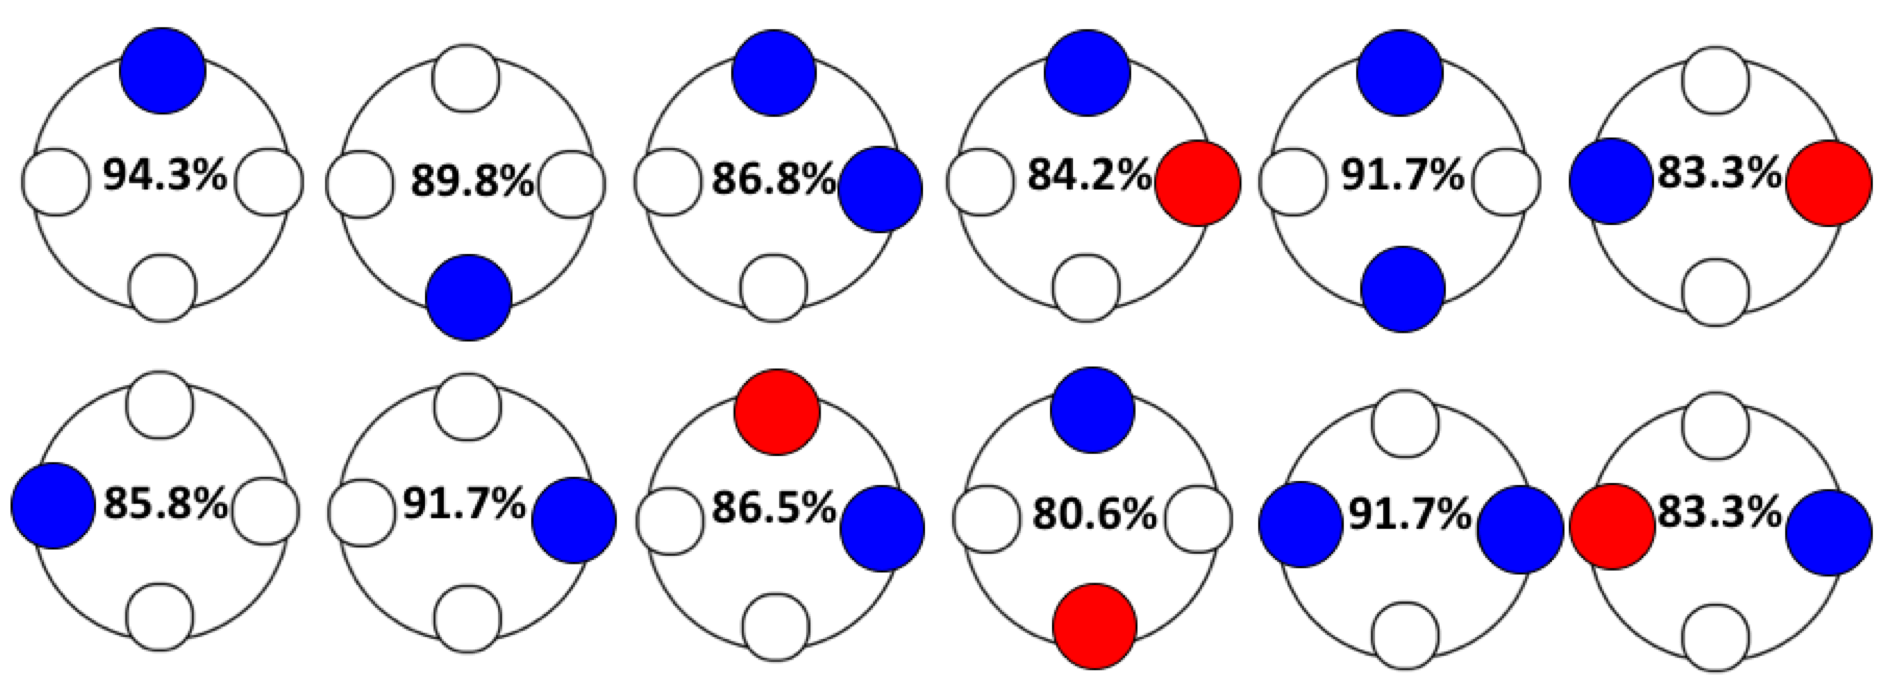
\includegraphics[width=0.9\columnwidth]{img/fig14.png}
  %\subfigure\cite{]{\label{fig:fold2}\includegraphics[width=0.45\textwidth]{images/wo_assembly.png}}
  \caption{The set of smart-ring thermal patterns that achieved above 80\% accuracy in the experiments.}
  \label{fig:14}
\end{figure}

Depending on the applications and needs, three more patterns could be included, which generally achieved more than 70\% accuracy: Bh, Th, and Rh. Note that we did not consider all the possible patterns for neighboring pairs. However, based on our pilot study that there is no significant difference between the accuracy of identifying the left and the right TECs, there might be other candidates with the Top+Left pair.

In general, it appears that a good spatial thermal pattern is more likely to get recognized if the distance between both TEC is maximum (i.e. using opposite pairs). Also, since it is easier to perceive a cold change, patterns with hot temperature change are discouraged.

\subsection{Cold vs. Hot Change}
While a hot temperature change may be convenient to encode a positive emotion \cite{41} or the general proximity to a point (e.g. ``you're getting hot'' to indicate that a person is getting closer to an objective) \cite{34}, the cold temperature change should be prioritized for information encoding. In-ring hot temperature change is more difficult to precisely locate, which impairs recognition. This could be further explained by the physiological fact that the density of  cold receptors is higher than warm receptors on the skin \cite{15}.

Additionally, during our experiments, seven participants reported an illusion of weight on the finger skin, feeling more heavily pressed with the hot temperature than with the cold temperature. This observation was contrary to the Weber's phenomenon \cite{4}, which reveals that a concomitantly cooling stimulus on hand will be perceived as significantly heavier than an identical stimulus of a neutral temperature. This contradiction could be explained by the non-uniformness of thermal perception across different body parts \cite{31}, indicating a need for a deeper investigation on user perception when designing smart ring thermal feedback.

\subsection{Applications Suggested by the Participants}
Besides emotion communication, which has been proved as a common application for thermal feedback, our participants suggested several new applications (e.g., directional cueing, notification, artefact comparison, and so on) which could be unique with our ring design. Furthermore, we have developed a set of proof-of-concept applications based on the new applications commonly suggested by the participants.

\subsubsection{Notifications}
Our set of 10-15 spatial thermal patterns, which can be perceived with the accuracy over 80\%, can be used as thermal icons to encode discrete notifications, similarly to any other modality. Our design leverages the simultaneous sensation of multiple TECs to achieve a rich expressivity that may not be obtainable with only one otherwise. Suggested by 18 participants, these unique spatial thermal patterns could be mapped to notifications from different applications, such as timer alarm, event reminder, incoming calls or messages from different persons or social networks. Previous research \cite{24} showed that users preferred the resistor-based in-ring thermal feedback for non-urgent or moderately urgent information updates. The average response time below 3s in our experiments further suggested the potential of using TEC-based in-ring spatial thermal patterns as the channel of notification. Fig. \ref{fig:15}a shows the in-ring thermal pattern (TcRc) indicating a call from an unknown number.

\subsubsection{Navigation}
Thirteen participants suggested that the neigboring patterns can be used as the directional cues. The neighboring patterns can encode the four cardinal directions: straight forward, left, right and go-back, using cold temperature change on one specific TEC, and the intermediate points between two consecutive cardinal directions, such as front-left and front-right, using two TEC modules. As revealed by Roumen et al. \cite{24}, our sensitivity to thermal stimuli on finger would increase with physical activity. These suggest a potential usage of the in-ring spatial thermal patterns as directional cues during physical activities (e.g. running and biking). Fig. \ref{fig:15}b shows the neighboring pattern of ThRc suggesting a front-left-left direction for biking.

\subsubsection{Comparison}
The reliable recognition of opposite thermal patterns supports artifact comparison through the difference of the temperatures on two TECs. Fig. \ref{fig:15}c shows the scenario of a user browsing an online bookstore. By selecting two books, the user toggles the comparison mode. Based on the spatial relation of the selected books (up-down/left-right arrangement), the ring automatically triggers the top-bottom/left-right thermal patterns. The higher temperature the representative TEC has, the more popular the book is. In a more futuristic scenario (Fig. \ref{fig:15}d), the user can compare two physical items, here the ratings of two movie DVDs, through the in-ring thermal patterns. This could be implemented by combining the in-ring TECs and in-ring camera or sensors.

\begin{figure}[tp]
  \centering
  %\subfigure\cite{]{\label{fig:fold1}\includegraphics[width=0.45\textwidth]{images/study_setup.png}}
  \includegraphics[width=0.8\columnwidth]{img/fig15.png}
  %\subfigure\cite{]{\label{fig:fold2}\includegraphics[width=0.45\textwidth]{images/wo_assembly.png}}
  \caption{Application scenarios for smart-ring thermal patterns: (a) notification, (b) navigation, (c) comparison of digital artifacts, (d) comparison of physical artifacts.}
  \label{fig:15}
\end{figure}

\subsection{Limitations}
We identified a few limitations and improvement space in our work during the experiments.

The current smart ring prototype is in a wearable and testable form factor but requires connection to an external control circuit. Our prototype shares the similar limitation of existing thermal research prototypes on being power consuming. For the simultaneous usage of multiple TECs, each requires 1.5W power.

Some participants reported an issue with direct skin contact with the hard TEC surface. While we allowed the participants to take time to adapt to the ring before starting the actual experiment, the hard surface of the TECs could be challenging for the prolonged use of the ring. Future work may need to consider the choice of thermally conductive soft material (e.g. sponge) to buffer the interface between the finger skin and the TEC surface.

We observed a difference in the thermal sensitivity among the participants. Medical research has demonstrated that the skin sensitivity could be affected by race, culture, and living region \cite{17}. We observed that all our participants were from the similar region and cultural background, thus could have similar skin sensitivity. In addition, it is implementable to allow users to customize the temperature change based on their own perception. We argue that our results in this paper would still be valid for other skin sensitivity when the temperature change is adjusted properly.

Furthermore, our study primarily focused on stimuli based on thermal parameters recommended from previous research \cite{42}: 1$^{\circ}$C/s for 3s, and the experiments were conducted with the participants sitting still indoor. While these factors ensured a perceivable and comfortable stimulus, there are more thermal parameters that could be adjusted for experimentation. Therefore, in our future studies, we wish to explore other variants of parameters such as the movement of participants, indoor/outdoor environments, rate of temperature change, stimulus duration, starting temperature, sequential temporal stimulation, etc., for smart-ring spatial thermal feedback.

\section{Conclusion and Future Work}
In this paper, we investigated smart ring thermal feedback with multiple TEC modules. In the pilot study, we showed that users could reliably recognize 4 locations with cold stimulation with 95.8\% accuracy, and achieve decent accuracy with hot stimulation (82.3\% accuracy). Further, we designed two types of spatial thermal patterns (neighboring and opposite) that can be achieved with 4 in-ring TECs. Experiments revealed 10 thermal patterns that can be reliably distinguished by participants, indicating their potential usage as in-ring thermal icons for notifications. Participants also elicited different applications, including direction cueing through neighboring patterns and artifact comparison through opposite patterns, demonstrating the interest of spatial thermal patterns in smart rings not only for notifications but also for various everyday activities. For future work, there is a need to investigate the effectiveness of the presented thermal patterns in different applications, such as emotion representation, notification, navigation, and comparison. Furthermore, we see the feasibility of integrating multiple feedback modalities (e.g. vibrotactile, poking, and thermal) in the form factor of a finger ring, and in investigating the interplay of multimodal feedback for smart ring.


\section*{Acknowledgement}
The work described in this paper was partially supported by the General Research Fund (Early Career Scheme) from the Research Grants Council of the Hong Kong Special Administrative Region, China (Project No. CityU 21200216), and the Strategic Research Grant (Project No. 7005021) from City University of Hong Kong.
%\label{}

%% The Appendices part is started with the command \appendix;
%% appendix sections are then done as normal sections
%% \appendix

%% \section{}
%% \label{}

%% If you have bibdatabase file and want bibtex to generate the
%% bibitems, please use
%%
%%  \bibliographystyle{elsarticle-num}
%%  \bibliography{<your bibdatabase>}

%% else use the following coding to input the bibitems directly in the
%% TeX file.
\section*{References}
\begin{thebibliography}{00}

%% \bibitem{label}
%% Text of bibliographic item
\bibitem{Alvina2015}
Jessalyn Alvina, Shengdong Zhao, Simon T. Perrault, Maryam Azh, Thijs Roumen, and Morten Fjeld. 2015. OmniVib: Towards Cross-body Spatiotemporal Vibrotactile Notifications for Mobile Phones. In Proceedings of the 33rd Annual ACM Conference on Human Factors in Computing Systems (CHI '15). ACM, New York, NY, USA, 2487-2496. DOI: https://doi.org/10.1145/2702123.2702341
\bibitem{Brown2005}
Brown, L. M., Brewster, S. A., and Purchase, H. C. 2005. A first investigation into the effectiveness of Tactons. In Proceedings of 1st Worldhaptics Conference (WHC '05), pp. 167-176, Pisa, Italy, March 2005.
\bibitem{1}
William S. Cain. 1973. Spatial Discrimination of Cutaneous Warmth. The American Journal of Psychology 86, 1: 169. https://doi.org/10.2307/1421858
\bibitem{2}
Marta G. Carcedo, Soon Hau Chua, Simon Perrault, Paweł Wozniak, Raj Joshi, Mohammad Obaid, Morten Fjeld, and Shengdong Zhao. 2016. HaptiColor. In Proceedings of the 2016 CHI Conference on Human Factors in Computing Systems - CHI '16, 3572-3583. https://doi.org/10.1145/2858036.2858220
\bibitem{3}
Jessica R. Cauchard, Janette L. Cheng, Thomas Pietrzak, and James A. Landay. 2016. ActiVibe: Design and Evaluation of Vibrations for Progress Monitoring. In Proceedings of the 2016 CHI Conference on Human Factors in Computing Systems - CHI '16, 3261-3271. https://doi.org/10.1145/2858036.2858046
\bibitem{Chan2008}
Chan, A., MacLean, K. E., and McGrenere, J. 2008. Designing haptic icons to support collaborative turn-taking. In Int'l J Human Computer Studies, vol. 66, pp. 333-355, January 2008. E-publication Nov 17, 2007.
\bibitem{PairRing}
Jungmin Chung, Changhoon Oh, SoHyun Park, and Bongwon Suh. 2018. PairRing: A Ring-Shaped Rotatable Smartwatch Controller. In Extended Abstracts of the 2018 CHI Conference on Human Factors in Computing Systems (CHI EA '18). ACM, New York, NY, USA, Paper LBW635, 6 pages. DOI: https://doi.org/10.1145/3170427.3188590
\bibitem{4}
James S. Dunn, David A. Mahns, and Saad S. Nagi. 2017. Why does a cooled object feel heavier? Psychophysical investigations into the Weber's Phenomenon. BMC Neuroscience 18, 4. https://doi.org/10.1186/s12868-016-0322-3
\bibitem{5}
Yuan-Ling Feng, Charith Lasantha Fernando, Jan Rod, and Kouta Minamizawa. 2017. Submerged haptics. In ACM SIGGRAPH 2017 Emerging Technologies on - SIGGRAPH '17, 1-2. https://doi.org/10.1145/3084822.3084835
\bibitem{Gallace2007}
Gallace, A., Tan, H. Z., and Spence, C. 2007. The body surface as a communication system: The state of the art after 50 years. In Presence: Teleoperators and Virtual Environments, vol. 16:6, pp. 655-676, December 2007.
\bibitem{Ringteraction}
Sarthak Ghosh, Hyeong Cheol Kim, Yang Cao, Arne Wessels, Simon T. Perrault, and Shengdong Zhao. 2016. Ringteraction: Coordinated Thumb-index Interaction Using a Ring. In Proceedings of the 2016 CHI Conference Extended Abstracts on Human Factors in Computing Systems (CHI EA '16). ACM, New York, NY, USA, 2640-2647. DOI: https://doi.org/10.1145/2851581.2892371
\bibitem{Gibson}
Gibson, G.O., Craig, J. C. Tactile spatial sensitivity and anisotropy. In Perception \& Psychophysics, vol. 67-6 (2005), 1061-1079.
\bibitem{6}
Barry G. Green. 1977. Localization of thermal sensation: An illusion and synthetic heat. Perception \& Psychophysics 22, 4: 331-337. https://doi.org/10.3758/BF03199698
\bibitem{7}
Martin Halvey, Michael Henderson, Stephen A. Brewster, Graham Wilson, and Stephen A. Hughes. 2012. Augmenting Media with Thermal Stimulation. . Springer, Berlin, Heidelberg, 91-100. https://doi.org/10.1007/978-3-642-32796-4\_10
\bibitem{8}
Martin Halvey, Graham Wilson, Stephen A. Brewster, and Stephen A. Hughes. 2012. Baby it's cold outside: the influence of ambient temperature and humidity on thermal feedback. Proceedings of the SIGCHI conference on Human factors in computing systems - CHI '12: 715-724. https://doi.org/10.1145/2207676.2207779
\bibitem{9}
Martin Halvey, Graham Wilson, Stephen A. Brewster, and Stephen A. Hughes. 2013. Perception of thermal stimuli for continuous interaction. In CHI '13 Extended Abstracts on Human Factors in Computing Systems on - CHI EA '13, 1587. https://doi.org/10.1145/2468356.2468640
\bibitem{10}
Martin Halvey, Graham Wilson, Yolanda Vazquez-Alvarez, Stephen A. Brewster, and Stephen A. Hughes. 2011. The effect of clothing on thermal feedback perception. In Proceedings of the 13th international conference on multimodal interfaces - ICMI '11, 217. https://doi.org/10.1145/2070481.2070519
\bibitem{11}
Teng Han, Qian Han, Michelle Annett, Fraser Anderson, Da-Yuan Huang, \& Xing-Dong Yang. 2017, October. Frictio: Passive Kinesthetic Force Feedback for Smart Ring Output. In Proceedings of the 30th Annual ACM Symposium on User Interface Software and Technology (pp. 131-142). ACM.
%TengHan, QianHan, MichelleAnnett, FraserAnderson, Da-YuanHuang, andXing-DongYang. 2017. Frictio: Passive Kinesthetic Force Feedback for Smart Ring Output. In Proceedings of UIST 2017. Retrieved September11, 2017 from http://hci.cs.umanitoba.ca/Publications/details/frictio-passive-kinesthetic-force-feedback-for-smart-ring-output
\bibitem{12}
Meng-Ju Hsieh, Rong-Hao Liang, and Bing-Yu Chen. 2016. NailTactors. In Proceedings of the 18th International Conference on Human-Computer Interaction with Mobile Devices and Services - MobileHCI '16, 29-34. https://doi.org/10.1145/2935334.2935358
\bibitem{13}
Seungwoo Je, Brendan Rooney, Liwei Chan, and Andrea Bianchi. 2017. tactoRing. In Proceedings of the 2017 CHI Conference on Human Factors in Computing Systems - CHI'17, 3106-3114. https://doi.org/10.1145/3025453.3025703
\bibitem{14}
Lynette A. Jones and Michal Berris. 2002. The psychophysics of temperature perception and thermal-interface design. In Proceedings - 10th Symposium on Haptic Interfaces for Virtual Environment and Teleoperator Systems, HAPTICS 2002, 137-142. https://doi.org/10.1109/HAPTIC.2002.998951
\bibitem{15}
Lynette A. Jones and Hsin Ni Ho. 2008. Warm or cool, large or small? The challenge of thermal displays. IEEE Transactions on Haptics 1, 1: 53-70. https://doi.org/10.1109/TOH.2008.2
\bibitem{16}
Joseph C. Stevens and Kenneth K. Choo. 1996. Spatial Acuity of the Body Surface over the Life Span. Somatosensory \& Motor Research 13, 2: 153-166. https://doi.org/10.3109/08990229609051403
\bibitem{MacLean2008}
MacLean, K. E. 2008. Foundations of Transparency in Tactile Information Design. IEEE Trans on Haptics, vol. 1:2, pp. 84-95, July-December 2008.
\bibitem{MacLean2003}
MacLean, K. E. and Enriquez, M.. 2003. Perceptual design of haptic icons. In Proceedings of EuroHaptics, pp. 351-363, Dublin, Ireland, Eurohaptics Society 2003.
\bibitem{Miller1956}
Miller, G. A. (1956). The magical number seven, plus or minus two: some limits on our capacity for processing information. Psychological Review, 63(2), 81-97. http://dx.doi.org/10.1037/h0043158
\bibitem{17}
Kenneth W. Miller, Abigail M. Wippel, Enzo Berardesca, Laurent Misery, and Howard Maibach. 2013. Sensitive Skin in the United States: Survey of Regional Differences. Family Medicine \& Medical Science Research 2, 3. https://doi.org/10.4172/2327-4972.1000112
\bibitem{18}
Lael U. Odhner and Haruhiko Harry Asada. 2006. Sensorless temperature estimation and control of shape memory alloy actuators using thermoelectric devices. IEEE/ASME Transactions on Mechatronics 11, 2: 139-144. https://doi.org/10.1109/TMECH.2006.871088
\bibitem{19}
Roshan Lalintha Peiris, Liwei Chan, and Kouta Minamizawa. 2016. Thermocons: Evaluating the Thermal Haptic Perception of the Forehead. In Proceedings of the 29th Annual Symposium on User Interface Software and Technology - UIST '16 Adjunct, 187-188. https://doi.org/10.1145/2984751.2984762
\bibitem{20}
Roshan Lalintha Peiris, Wei Peng, Zikun Chen, Liwei Chan, and Kouta Minamizawa. 2017. ThermoVR. In Proceedings of the 2017 CHI Conference on Human Factors in Computing Systems - CHI '17, 5452-5456. https://doi.org/10.1145/3025453.3025824
\bibitem{OctaRing}
Hyunchul Lim, Jungmin Chung, Changhoon Oh, SoHyun Park, and Bongwon Suh. 2016. OctaRing: Examining Pressure-Sensitive Multi-Touch Input on a Finger Ring Device. In Proceedings of the 29th Annual Symposium on User Interface Software and Technology (UIST '16 Adjunct). ACM, New York, NY, USA, 223-224. DOI: https://doi.org/10.1145/2984751.2984780
\bibitem{Machado2008}
Machado-Moreira, Christiano A. and Caldwell, Joanne N. and Mekjavic, Igor B. and Taylor, Nigel A. S. 2008. Sweat Secretion from Palmar and Dorsal Surfaces of the Hands During Passive and Active Heating. In Aviation, Space, and Environmental Medicine 79, 11:1034-1040.
\bibitem{21}
Doros Polydorou, Kening Zhu, and Alexis Karkotis. 2017. Digital Humanities and Techno-Animism in Wearables: A Case-Study-Based Collaborative Design Framework for Digitally-Ensouled Jewellery. . Springer, Cham, 719-736. https://doi.org/10.1007/978-3-319-58637-3\_55
\bibitem{22}
Gilang Andi Pradana, Adrian David Cheok, Masahiko Inami, Jordan Tewell, and Yongsoon Choi. 2014. Emotional priming of mobile text messages with ring-shaped wearable device using color lighting and tactile expressions. In Proceedings of the 5th Augmented Human International Conference, 14.
\bibitem{23}
Nimesha Ranasinghe, Pravar Jain, Shienny Karwita, David Tolley, and Ellen Yi-Luen Do. 2017. Ambiotherm. In Proceedings of the 2017 CHI Conference on Human Factors in Computing Systems - CHI '17, 1731-1742. https://doi.org/10.1145/3025453.3025723
\bibitem{24}
Thijs Roumen, Simon T. Perrault, and Shengdong Zhao. 2015. NotiRing: A Comparative Study of Notification Channels for Wearable Interactive Rings. In Proceedings of the 33rd Annual ACM Conference on Human Factors in Computing Systems - CHI '15, 2497-2500. https://doi.org/10.1145/2702123.2702350
\bibitem{25}
Bahador Saket, Chrisnawan Prasojo, Yongfeng Huang, and Shengdong Zhao. 2013. Designing an effective vibration-based notification interface for mobile phones. In Proceedings of the 2013 conference on Computer supported cooperative work - CSCW '13, 149. https://doi.org/10.1145/2441776.2441946
\bibitem{26}
Katsunari Sato and Takashi Maeno. 2012. Presentation of Sudden Temperature Change Using Spatially Divided Warm and Cool Stimuli. . Springer, Berlin, Heidelberg, 457-468. https://doi.org/10.1007/978-3-642-31401-8\_41
\bibitem{27}
Anshul Singhal and Lynette Jones. 2016. Space-Time Dependencies and Thermal Perception. . Springer, Cham, 291-302. https://doi.org/10.1007/978-3-319-42321-0\_27
\bibitem{28}
Joseph C. Stevens. 1982. Temperature can sharpen tactile acuity. Perception \& Psychophysics 31, 6: 577-580. https://doi.org/10.3758/BF03204192
\bibitem{29}
Joseph C. Stevens. 1989. Temperature and the Two-Point Threshold. Somatosensory \& Motor Research 6, 3: 275-284. https://doi.org/10.3109/08990228909144677
\bibitem{30}
Joseph C. Stevens, Lawrence E. Marks, and Donald C. Simonson. 1974. Regional sensitivity and spatial summation in the warmth sense. Physiology \& Behavior 13, 6: 825-836. https://doi.org/10.1016/0031-9384(74)90269-8
\bibitem{31}
Josepth C. Stevens and Kenneth K. Choo. 1998. Temperature sensitivity of the body surface over the life span. Somatosensory \& Motor Research 15, 1: 13-28. https://doi.org/10.1080/08990229870925
\bibitem{32}
Murakami Takaki, Person Tanner, Fernando Charith, and Minamizawa Kouta. 2017. Altered Touch�: Miniature Haptic Display with Force , Thermal and Tactile Feedback for Augmented Haptics. In SIGGRAPH 2017, 1-2. https://doi.org/10.1145/3084822.3084836
\bibitem{33}
Richard H. Taus, Joseph C. Stevens, and Lawrence E. Marks. 1975. Spatial localization of warmth. Perception \& Psychophysics 17, 2: 194-196. https://doi.org/10.3758/BF03203885
\bibitem{34}
Jordan Tewell, Jon Bird, and George R. Buchanan. 2017. Heat-Nav: Using Temperature Changes as Navigational Cues. Proceedings of the 2017 CHI Conference on Human Factors in Computing Systems - CHI '17: 1131-1135. https://doi.org/10.1145/3025453.3025965
\bibitem{35}
Jordan Tewell, Jon Bird, and George R. Buchanan. 2017. The Heat is On. Proceedings of the 2017 CHI Conference on Human Factors in Computing Systems - CHI '17: 1756-1767. https://doi.org/10.1145/3025453.3025844
\bibitem{36}
Reto Wettach, Christian Behrens, Adam Danielsson, and Thomas Ness. 2007. A thermal information display for mobile applications. In Proceedings of the 9th international conference on Human computer interaction with mobile devices and services - MobileHCI '07, 182-185. https://doi.org/10.1145/1377999.1378004
\bibitem{37}
Graham Wilson and Stephen A. Brewster. 2017. Multi-Moji: Combining Thermal, Vibrotactile \& Visual Stimuli to Expand the Affective Range of Feedback. In CHI '17 Proceedings of the 2017 CHI Conference on Human Factors in Computing Systems, 1742-1755. https://doi.org/10.1145/3025453.3025614
\bibitem{38}
Graham Wilson, Stephen A. Brewster, Martin Halvey, and Stephen A. Hughes. 2012. Thermal Icons: Evaluating Structured Thermal Feedback for Mobile Interaction. Proceedings of the 14th international conference on Human-computer interaction with mobile devices and services - MobileHCI'12: 309-312. https://doi.org/10.1145/2371574.2371621
\bibitem{39}
Graham Wilson, Stephen Brewster, Martin Halvey, and Stephen Hughes. 2013. Thermal Feedback Identification in a Mobile Environment. . Springer, Berlin, Heidelberg, 10-19. https://doi.org/10.1007/978-3-642-41068-0\_2
\bibitem{40}
Graham Wilson, Gavin Davidson, and Stephen A. Brewster. 2015. In the Heat of the Moment. In Proceedings of the 33rd Annual ACM Conference on Human Factors in Computing Systems - CHI '15, 2063-2072. https://doi.org/10.1145/2702123.2702219
\bibitem{41}
Graham Wilson, Dobromir Dobrev, and Stephen A. Brewster. 2016. Hot Under the Collar. In Proceedings of the 2016 CHI Conference on Human Factors in Computing Systems - CHI '16, 4838-4849. https://doi.org/10.1145/2858036.2858205
\bibitem{42}
Graham Wilson, Martin Halvey, Stephen A. Brewster, and Stephen A. Hughes. 2011. Some Like it Hot: Thermal Feedback for Mobile Devices. In Proceedings of the SIGCHI conference on Human Factors in Computing Systems - CHI '11, 2555-2564. https://doi.org/10.1145/1978942.1979316
\bibitem{43}
G.-H. Yang, D.-S. Kwon, and L. A.Jones. 2009. Spatial acuity and summation on the hand: The role of thermal cues in material discrimination. Perception \& Psychophysics 71, 1: 156-163. https://doi.org/10.3758/APP.71.1.156
\bibitem{Semfeel}
Yatani, K., Truong, K.N. 2009. SemFeel: a user interface with semantic tactile feedback for mobile touch-screen devices. In Proc. UIST 2009. ACM (2009), 111-120.
\bibitem{44}
Vibol Yem, Ryuta Okazaki, and Hiroyuki Kajimoto. 2016. FinGAR. In ACM SIGGRAPH 2016 Emerging Technologies on - SIGGRAPH '16, 1-2. https://doi.org/10.1145/2929464.2929474
\bibitem{45}
Hui Zhang, Edward Arens, Charlie Huizenga, and Taeyoung Han. 2010. Thermal sensation and comfort models for non-uniform and transient environments: Part I: Local sensation of individual body parts. Building and Environment 45, 2: 380-388. https://doi.org/10.1016/j.buildenv.2009.06.018

%\bibitem{1}
%William S. Cain. 1973. Spatial Discrimination of Cutaneous Warmth. The American Journal of Psychology 86, 1: 169.
%
%\bibitem{2}
%Marta G. Carcedo, Soon Hau Chua, Simon Perrault, Paweł Wozniak, Raj Joshi, Mohammad Obaid, Morten Fjeld, and Shengdong Zhao. 2016. HaptiColor. In Proceedings of the 2016 CHI Conference on Human Factors in Computing Systems - CHI '16, 3572–3583.
%
%\bibitem{3}
%Jessica R. Cauchard, Janette L. Cheng, Thomas Pietrzak, and James A. Landay. 2016. ActiVibe: Design and Evaluation of Vibrations for Progress Monitoring. In Proceedings of the 2016 CHI Conference on Human Factors in Computing Systems - CHI '16, 3261–3271.
%
%\bibitem{4}
%James S. Dunn, David A. Mahns, and Saad S. Nagi. 2017. Why does a cooled object feel heavier? Psychophysical investigations into the Weber’s Phenomenon. BMC Neuroscience 18, 4.
%
%\bibitem{5}
%Yuan-Ling Feng, Charith Lasantha Fernando, Jan Rod, and Kouta Minamizawa. 2017. Submerged haptics. In ACM SIGGRAPH 2017 Emerging Technologies on - SIGGRAPH '17, 1–2.
%
%\bibitem{6}
%Martin Halvey, Michael Henderson, Stephen A. Brewster, Graham Wilson, and Stephen A. Hughes. 2012. Augmenting Media with Thermal Stimulation. . Springer, Berlin, Heidelberg, 91–100.
%
%\bibitem{7}
%Martin Halvey, Graham Wilson, Stephen A. Brewster, and Stephen A. Hughes. 2012. Baby it’s cold outside: the influence of ambient temperature and humidity on thermal feedback. Proceedings of the SIGCHI conference on Human factors in computing systems - CHI '12: 715–724.
%
%\bibitem{8}
%Martin Halvey, Graham Wilson, Stephen A. Brewster, and Stephen A. Hughes. 2013. Perception of thermal stimuli for continuous interaction. In CHI '13 Extended Abstracts on Human Factors in Computing Systems on - CHI EA '13, 1587.
%
%\bibitem{9}
%Martin Halvey, Graham Wilson, Yolanda Vazquez-Alvarez, Stephen A. Brewster, and Stephen A. Hughes. 2011. The effect of clothing on thermal feedback perception. In Proceedings of the 13th international conference on multimodal interfaces - ICMI '11, 217.
%
%\bibitem{10}
%Teng Han, Qian Han, Michelle Annett, Fraser Anderson, Da-Yuan Huang, and Xing-Dong Yang. 2017. Frictio: Passive Kinesthetic Force Feedback for Smart Ring Output. In Proceedings of UIST 2017.
%
%\bibitem{11}
%Meng-Ju Hsieh, Rong-Hao Liang, and Bing-Yu Chen. 2016. NailTactors. In Proceedings of the 18th International Conference on Human-Computer Interaction with Mobile Devices and Services - MobileHCI '16, 29–34.
%
%\bibitem{12}
%Seungwoo Je, Brendan Rooney, Liwei Chan, and Andrea Bianchi. 2017. tactoRing. In Proceedings of the 2017 CHI Conference on Human Factors in Computing Systems - CHI '17, 3106–3114.
%
%\bibitem{13}
%Lynette A. Jones and Michal Berris. 2002. The psychophysics of temperature perception and thermal-interface design. In Proceedings - 10th Symposium on Haptic Interfaces for Virtual Environment and Teleoperator Systems, HAPTICS 2002, 137–142.
%
%\bibitem{14}
%Lynette A. Jones and Hsin Ni Ho. 2008. Warm or cool, large or small? The challenge of thermal displays. IEEE Transactions on Haptics 1, 1: 53–70.
%
%\bibitem{15}
%Kenneth W. Miller, Abigail M. Wippel, Enzo Berardesca, Laurent Misery, and Howard Maibach. 2013. Sensitive Skin in the United States: Survey of Regional Differences. Family Medicine \& Medical Science Research 2, 3.
%
%\bibitem{16}
%Lael U. Odhner and Haruhiko Harry Asada. 2006. Sensorless temperature estimation and control of shape memory alloy actuators using thermoelectric devices. IEEE/ASME Transactions on Mechatronics 11, 2: 139–144.
%
%\bibitem{17}
%Roshan Lalintha Peiris, Liwei Chan, and Kouta Minamizawa. 2016. Thermocons: Evaluating the Thermal Haptic Perception of the Forehead. In Proceedings of the 29th Annual Symposium on User Interface Software and Technology - UIST '16 Adjunct, 187–188.
%
%\bibitem{18}
%Roshan Lalintha Peiris, Wei Peng, Zikun Chen, Liwei Chan, and Kouta Minamizawa. 2017. ThermoVR. In Proceedings of the 2017 CHI Conference on Human Factors in Computing Systems - CHI '17, 5452–5456.
%
%\bibitem{19}
%Doros Polydorou, Kening Zhu, and Alexis Karkotis. 2017. Digital Humanities and Techno-Animism in Wearables: A Case-Study-Based Collaborative Design Framework for Digitally-Ensouled Jewellery. Springer, Cham, 719–736.
%
%\bibitem{20}
%Gilang Andi Pradana, Adrian David Cheok, Masahiko Inami, Jordan Tewell, and Yongsoon Choi. 2014. Emotional priming of mobile text messages with ring-shaped wearable device using color lighting and tactile expressions. In Proceedings of the 5th Augmented Human International Conference, 14.
%
%\bibitem{21}Nimesha Ranasinghe, Pravar Jain, Shienny Karwita, David Tolley, and Ellen Yi-Luen Do. 2017. Ambiotherm. In Proceedings of the 2017 CHI Conference on Human Factors in Computing Systems - CHI '17, 1731–1742.
%
%\bibitem{22}
%Thijs Roumen, Simon T. Perrault, and Shengdong Zhao. 2015. NotiRing: A Comparative Study of Notification Channels for Wearable Interactive Rings. In Proceedings of the 33rd Annual ACM Conference on Human Factors in Computing Systems - CHI '15, 2497–2500.
%
%\bibitem{23}
%Bahador Saket, Chrisnawan Prasojo, Yongfeng Huang, and Shengdong Zhao. 2013. Designing an effective vibration-based notification interface for mobile phones. In Proceedings of the 2013 conference on Computer supported cooperative work - CSCW '13, 149.
%
%\bibitem{24}
%Katsunari Sato and Takashi Maeno. 2012. Presentation of Sudden Temperature Change Using Spatially Divided Warm and Cool Stimuli. . Springer, Berlin, Heidelberg, 457–468.
%
%\bibitem{25}
%Anshul Singhal and Lynette Jones. 2016. Space-Time Dependencies and Thermal Perception. . Springer, Cham, 291–302.
%
%\bibitem{255}
%Josepth C. Stevens. 1989. Temperature and the two-point threshold. Somatosensory \& motor research, 6, 3: 275-284.
%
%\bibitem{26}
%Josepth C. Stevens and Kenneth K. Choo. 1996. Spatial Acuity of the Body Surface over the Life Span. Somatosensory \& Motor Research 13, 2: 153–166.
%
%\bibitem{27}
%Josepth C. Stevens and Kenneth K. Choo. 1998. Temperature sensitivity of the body surface over the life span. Somatosensory \& Motor Research 15, 1: 13–28.
%
%\bibitem{28}
%Murakami Takaki, Person Tanner, Fernando Charith, and Minamizawa Kouta. 2017. Altered Touch : Miniature Haptic Display with Force , Thermal and Tactile Feedback for Augmented Haptics. In SIGGRAPH 2017, 1–2.
%
%\bibitem{29}
%Richard H. Taus, Joseph C. Stevens, and Lawrence E. Marks. 1975. Spatial localization of warmth. Perception \& Psychophysics 17, 2: 194–196.
%
%\bibitem{30}
%Jordan Tewell, Jon Bird, and George R. Buchanan. 2017. Heat-Nav: Using Temperature Changes as Navigational Cues. Proceedings of the 2017 CHI Conference on Human Factors in Computing Systems - CHI '17: 1131–1135.
%
%\bibitem{31}
%Jordan Tewell, Jon Bird, and George R. Buchanan. 2017. The Heat is On. Proceedings of the 2017 CHI Conference on Human Factors in Computing Systems - CHI '17: 1756–1767.
%
%\bibitem{32}
%Reto Wettach, Christian Behrens, Adam Danielsson, and Thomas Ness. 2007. A thermal information display for mobile applications. In Proceedings of the 9th international conference on Human computer interaction with mobile devices and services - MobileHCI '07, 182–185.
%
%\bibitem{33}
%Graham Wilson and Stephen A. Brewster. 2017. Multi-Moji: Combining Thermal, Vibrotactile \& Visual Stimuli to Expand the Affective Range of Feedback. In CHI '17 Proceedings of the 2017 CHI Conference on Human Factors in Computing Systems, 1742–1755.
%
%\bibitem{34}
%Graham Wilson, Stephen A. Brewster, Martin Halvey, and Stephen A. Hughes. 2012. Thermal Icons: Evaluating Structured Thermal Feedback for Mobile Interaction. Proceedings of the 14th international conference on Human-computer interaction with mobile devices and services - MobileHCI’12: 309–312.
%
%\bibitem{35}
%Graham Wilson, Stephen Brewster, Martin Halvey, and Stephen Hughes. 2013. Thermal Feedback Identification in a Mobile Environment. . Springer, Berlin, Heidelberg, 10–19.
%
%\bibitem{36}
%Graham Wilson, Gavin Davidson, and Stephen A. Brewster. 2015. In the Heat of the Moment. In Proceedings of the 33rd Annual ACM Conference on Human Factors in Computing Systems - CHI '15, 2063–2072.
%
%\bibitem{37}
%Graham Wilson, Dobromir Dobrev, and Stephen A. Brewster. 2016. Hot Under the Collar. In Proceedings of the 2016 CHI Conference on Human Factors in Computing Systems - CHI '16, 4838–4849.
%
%\bibitem{38}
%Graham Wilson, Martin Halvey, Stephen A. Brewster, and Stephen A. Hughes. 2011. Some Like it Hot: Thermal Feedback for Mobile Devices. In Proceedings of the SIGCHI conference on Human Factors in Computing Systems - CHI '11, 2555–2564.
%
%\bibitem{39}
%Vibol Yem, Ryuta Okazaki, and Hiroyuki Kajimoto. 2016. FinGAR. In ACM SIGGRAPH 2016 Emerging Technologies on - SIGGRAPH '16, 1–2.
%
%\bibitem{40}
%Hui Zhang, Edward Arens, Charlie Huizenga, and Taeyoung Han. 2010. Thermal sensation and comfort models for non-uniform and transient environments: Part I: Local sensation of individual body parts. Building and Environment 45, 2: 380–388.



%\bibitem{Stevens1996}
%Josepth C. Stevens and Kenneth K. Choo. 1996. Spatial Acuity of the Body Surface over the Life Span. \textit{Somatosensory \& Motor Research}. 13, 2: 153–166.

%\bibitem{Cauchard2016}
%Jessica R. Cauchard, Janette L. Cheng, Thomas Pietrzak, and James A. Landay. 2016. ActiVibe: Design and Evaluation of Vibrations for Progress Monitoring. In \textit{Proceedings of the 2016 CHI Conference on Human Factors in Computing Systems - CHI ’16}, 3261–3271.



\end{thebibliography}

\end{document}

\endinput
%%
%% End of file `elsarticle-template-num.tex'.
